%%
%% This is file `sample-sigconf.tex',
%% generated with the docstrip utility.
%%
%% The original source files were:
%%
%% samples.dtx  (with options: `all,proceedings,bibtex,sigconf')
%% 
%% IMPORTANT NOTICE:
%% 
%% For the copyright see the source file.
%% 
%% Any modified versions of this file must be renamed
%% with new filenames distinct from sample-sigconf.tex.
%% 
%% For distribution of the original source see the terms
%% for copying and modification in the file samples.dtx.
%% 
%% This generated file may be distributed as long as the
%% original source files, as listed above, are part of the
%% same distribution. (The sources need not necessarily be
%% in the same archive or directory.)
%%
%%
%% Commands for TeXCount
%TC:macro \cite [option:text,text]
%TC:macro \citep [option:text,text]
%TC:macro \citet [option:text,text]
%TC:envir table 0 1
%TC:envir table* 0 1
%TC:envir tabular [ignore] word
%TC:envir displaymath 0 word
%TC:envir math 0 word
%TC:envir comment 0 0
%%
%% The first command in your LaTeX source must be the \documentclass
%% command.
%%
%% For submission and review of your manuscript please change the
%% command to \documentclass[manuscript, screen, review]{acmart}.
%%
%% When submitting camera ready or to TAPS, please change the command
%% to \documentclass[sigconf]{acmart} or whichever template is required
%% for your publication.
%%
%%
\documentclass[sigconf]{acmart}
%%
%% \BibTeX command to typeset BibTeX logo in the docs
\AtBeginDocument{%
  \providecommand\BibTeX{{%
    Bib\TeX}}}

%% Rights management information.  This information is sent to you
%% when you complete the rights form.  These commands have SAMPLE
%% values in them; it is your responsibility as an author to replace
%% the commands and values with those provided to you when you
%% complete the rights form.
\setcopyright{acmlicensed}
\copyrightyear{2018}
\acmYear{2018}
\acmDOI{XXXXXXX.XXXXXXX}
%% These commands are for a PROCEEDINGS abstract or paper.
\acmConference[Conference acronym 'XX]{Make sure to enter the correct
  conference title from your rights confirmation email}{June 03--05,
  2018}{Woodstock, NY}
%%
%%  Uncomment \acmBooktitle if the title of the proceedings is different
%%  from ``Proceedings of ...''!
%%
%%\acmBooktitle{Woodstock '18: ACM Symposium on Neural Gaze Detection,
%%  June 03--05, 2018, Woodstock, NY}
\acmISBN{978-1-4503-XXXX-X/2018/06}













% themis red comment
\newcommand{\tp}[1]{\textcolor{red}{{\bf[$^{Themis: }$ ??? #1 ???]}}}




\newcommand{\ch}[1]{{\color{magenta} \noindent \textbf{ [Christos] #1}}\normalcolor}


\newcommand{\newContent}[1]{{\color{blue} #1}\normalcolor}










%%
%% Submission ID.
%% Use this when submitting an article to a sponsored event. You'll
%% receive a unique submission ID from the organizers
%% of the event, and this ID should be used as the parameter to this command.
%%\acmSubmissionID{123-A56-BU3}

%%
%% For managing citations, it is recommended to use bibliography
%% files in BibTeX format.
%%
%% You can then either use BibTeX with the ACM-Reference-Format style,
%% or BibLaTeX with the acmnumeric or acmauthoryear sytles, that include
%% support for advanced citation of software artefact from the
%% biblatex-software package, also separately available on CTAN.
%%
%% Look at the sample-*-biblatex.tex files for templates showcasing
%% the biblatex styles.
%%

%%
%% The majority of ACM publications use numbered citations and
%% references.  The command \citestyle{authoryear} switches to the
%% "author year" style.
%%
%% If you are preparing content for an event
%% sponsored by ACM SIGGRAPH, you must use the "author year" style of
%% citations and references.
%% Uncommenting
%% the next command will enable that style.
%%\citestyle{acmauthoryear}

\usepackage{float}
\usepackage{pgffor} % Package needed for loops
\usepackage{graphicx}
\usepackage{subcaption} % For handling subfigures
\usepackage{caption}
\usepackage{pgffor} % for \foreach
\usepackage{xstring}
\captionsetup{labelfont=normalfont, textfont=normalfont}
%%
%% end of the preamble, start of the body of the document source.
\renewcommand{\abstractname}{\textsc{Abstract}}

\begin{document}

%%
%% The "title" command has an optional parameter,
%% allowing the author to define a "short title" to be used in page headers.
% \title{A Comprehensive Survey and Evaluation on the High-Dimensional Vector Compression Techniques}
\title{A Systematic Benchmark of High-Dimensional Vector Compression Methods}
%%
%% The "author" command and its associated commands are used to define
%% the authors and their affiliations.
%% Of note is the shared affiliation of the first two authors, and the
%% "authornote" and "authornotemark" commands
%% used to denote shared contribution to the research.
 \author{Christos Panourgias}
% %\authornote{Both authors contributed equally to this research.}
 \email{panourgiaschris@gmail.com}
% %\orcid{1234-5678-9012}
% \author{Qitong Wang}
% %\authornotemark[1]
% \email{XXXXXXXXX}
% \author{Themis Palpanas}
% \email{themis@mi.parisdescartes.fr}
 \affiliation{%
   \institution{LIPADE, Universit{\'e} Paris Cit{\'e}}
  % \streetaddress{P.O. Box 1212}
  % \city{Dublin}
  % \state{Ohio}
   \country{France}
  % \postcode{43017-6221}
}

 \author{Shen Liang}
 \email{XXXXXXXXXXXXXXXX}
 \affiliation{%
   \institution{XXXXXXXXXXXXXXXX}
%   \city{Rocquencourt}
   \country{xxx}
}


 \author{Zeyu Wang}
 \email{zeyuwang21@m.fudan.edu.cn}
 \affiliation{%
   \institution{Fudan University}
%   \city{Rocquencourt}
   \country{China}
}

 \author{Yanlin Qi}
 \email{XXXXXXXXXXXXXXXX}
 \affiliation{%
   \institution{XXXXXXXXXXXXXXXX}
%   \city{Rocquencourt}
   \country{xxx}
}

 \author{Qitong Wang}
 \email{XXXXXXXXXXXXXXXX}
 \affiliation{%
   \institution{XXXXXXXXXXXXXXXX}
%   \city{Rocquencourt}
   \country{xxx}
}
 \author{Botao Peng}
 \email{pengbotao@ict.ac.cn}
  \affiliation{%
   \institution{Institute of Computing Technology, Chinese Academy of Sciences
   }
   \country{China}
   }

 \author{Themis Palpanas}
 \email{themis@mi.parisdescartes.fr}
 \affiliation{%
   \institution{LIPADE, Universit{\'e} Paris Cit{\'e}}
%   \city{Rocquencourt}
   \country{France}
}

   

%   \city{Rocquencourt}
%   \country{France}

%  \author{Nick Koudas}
%  \email{XXXXXXXXXXXXX}
%  \affiliation{%
%   \institution{University of Toronto}
% %  \streetaddress{Rono-Hills}
% %  \city{Doimukh}
% %  \state{Arunachal Pradesh}
% %  \country{India}
% }

%%
%% By default, the full list of authors will be used in the page
%% headers. Often, this list is too long, and will overlap
%% other information printed in the page headers. This command allows
%% the author to define a more concise list
%% of authors' names for this purpose.
\renewcommand{\shortauthors}{Panourgias et al.}

%%
%% The abstract is a short summary of the work to be presented in the
%% article.
\begin{abstract}
High-dimensional vector compression has become a key enabler for efficient machine learning at scale. The rapid growth of foundation models and large language models has increased both the volume of training data and the reliance on embedding-based workflows, where compact vector representations are critical for reducing storage and accelerating operations such as similarity search over large databases. In this work, we conduct a systematic study of high-dimensional vector compression methods. We benchmark them under a unified evaluation protocol and analyze how their performance varies with method-specific hyperparameters, highlighting trade-offs that are often obscured by default settings. We report results across compression quality and efficiency metrics, including reconstruction distortion, index size, encoding/decoding cost, and downstream retrieval performance. Our findings provide practical guidance for selecting and tuning compression techniques under different accuracy–latency–memory constraints, and establish a reproducible baseline for future research in large-scale vector retrieval and representation learning. 

\end{abstract}




%%
%% The code below is generated by the tool at http://dl.acm.org/ccs.cfm.
%% Please copy and paste the code instead of the example below.
%%


%%
%% This command processes the author and affiliation and title
%% information and builds the first part of the formatted document.
\maketitle
\section{Introduction}

High-dimensional vector representations have become a core data type in modern data management and machine learning systems. 
Dense embeddings produced by neural models are widely used to represent text, images, users, items, and other complex objects, supporting applications such as semantic search, recommendation, retrieval-augmented generation, clustering, classification, and scientific data analysis~\cite{huang2020embedding,rec2,lewis2020rag,gao2023ragsurvey}. 
The practical importance of this abstraction is reflected in modern vector data management systems, which are designed to store, index, and query large collections of embedding vectors~\cite{milvus,manu,adbv,vbase}. 
As embedding models and vector databases continue to scale, systems must increasingly operate over collections containing millions to billions of high-dimensional vectors. 
This makes vector storage and distance computation major bottlenecks in terms of memory footprint, query latency, bandwidth consumption, and energy cost.

Approximate Nearest-Neighbor Search (ANNS) has become the dominant approach for large-scale vector retrieval because exact search is often too expensive in high-dimensional spaces~\cite{tkde-survey,ann-benchmark,hnsw,faiss}. 
However, even within ANNS pipelines, distance computation remains a central cost, since common similarity measures such as Euclidean distance and inner product scale linearly with vector dimensionality~\cite{adsampling,dco,wang2024dimensionality}. 
At the same time, raw high-dimensional embeddings often dominate the memory footprint of vector indexes. 
These two pressures make vector compression an essential systems primitive for scalable vector data management.

In this work, we use \emph{Vector Compression} as an umbrella term for methods that replace high-dimensional floating-point vectors with compact representations while preserving their utility for similarity computation. 
Classical vector quantization methods, such as product quantization, optimized product quantization, residual quantization, additive quantization, and local-search-based multi-codebook quantization, have been widely used to reduce storage and support approximate distance computation from compact codes~\cite{pq,opq,rq,lsq,lsq++}. 
Recent methods extend this design space with adaptive bit allocation, randomized quantization with theoretical guarantees, online coordinate quantization, segmented quantization, and neural residual quantizers~\cite{vaq,rabitq,zandieh2025turboquant,li2025saq,qinco1,qinco2}. 
Projection, hashing, and learned low-dimensional representations provide another family of approaches for reducing the cost of similarity computation~\cite{lsh,pmlsh,wang2024dimensionality,seanet}. 
Although these techniques differ substantially in their design, they share the same practical goal: reducing the cost of operating over large vector collections while preserving the geometric relationships needed by downstream applications.

Despite the importance of vector compression, its empirical behavior remains difficult to understand and compare. 
Most existing benchmarks and experimental studies evaluate compression as one component inside a complete ANNS pipeline~\cite{ann-benchmark,competition,tkde-survey,wang-survey,ilias-benchmark,martin-survey}. 
Such end-to-end evaluations are useful, but they conflate several effects: the quality of the compressed representation, the index structure, candidate-generation strategy, pruning heuristic, reranking policy, implementation optimizations, and hardware-specific behavior. 
As a result, when one system outperforms another, it is often unclear whether the improvement comes from the compression method itself or from the surrounding search pipeline. 
Conversely, a compression method that performs poorly inside one index may be effective under a different retrieval architecture or memory budget.

A second difficulty is that vector compression methods are often evaluated using different objectives and metrics. 
Some methods optimize reconstruction distortion, others optimize distance estimation, inner-product preservation, ranking quality, or downstream recall. 
However, these metrics are not interchangeable: low reconstruction error does not necessarily imply accurate distance estimates, and accurate average distance estimates may still fail to preserve nearest-neighbor rankings~\cite{scann,rabitq,li2025saq}. 
Similarly, a method with high recall may require expensive decoding or reranking, while another method may offer lower accuracy but substantially better compressed-domain distance computation. 
A fair benchmark must therefore separate compression-intrinsic metrics, such as distance error and rank preservation, from downstream retrieval metrics, such as recall and query latency.

A third challenge is parameter sensitivity. 
Many compression methods expose several hyperparameters: code length, number of subquantizers, number of centroids, residual depth, projection dimensionality, number of bits per dimension, segmentation strategy, training set size, and search-time refinement budget. 
These parameters can drastically change the accuracy--latency--memory trade-off. 
Nevertheless, many prior comparisons rely on default settings or method-specific configurations, making it difficult to determine whether observed differences reflect fundamental method behavior or tuning choices. 
For practitioners, this creates a practical question: given a target memory budget and latency constraint, which compression method should be selected, and how should it be configured?

This paper addresses these issues through a systematic benchmark of high-dimensional vector compression methods. 
Rather than treating compression only as an internal component of a specific ANNS index, we evaluate compression as a first-class object of study. 
Our benchmark is designed around two complementary levels. 
First, we perform an \emph{intrinsic} evaluation of compression quality, measuring how well compressed representations preserve distances, rankings, reconstruction quality, storage efficiency, encoding cost, and compressed-domain distance computation time. 
Second, we evaluate how these compression properties translate to downstream retrieval performance under controlled search workloads. 
This two-level design allows us to isolate the behavior of compression methods while still assessing their practical impact on vector search systems.

Concretely, this paper asks the following questions:

\begin{itemize}
    \item \textbf{RQ1: Distance preservation.} 
    How accurately do different compression families preserve Euclidean distances under equal memory budgets?

    \item \textbf{RQ2: Ranking preservation.} 
    To what extent do compressed distances preserve nearest-neighbor orderings, and how does this relate to distance error?

    \item \textbf{RQ3: Efficiency trade-offs.} 
    How do compression accuracy, encoding time, decoding time, and compressed-domain distance computation time trade off?

    \item \textbf{RQ4: Parameter sensitivity.} 
    Which hyperparameters dominate performance, and are commonly used default settings reliable across datasets?

    \item \textbf{RQ5: Downstream impact.} 
    Do compression-level metrics predict retrieval quality, and which methods are preferable under different accuracy--latency--memory constraints?
\end{itemize}

To answer these questions, we benchmark representative methods from several families of vector compression, including product quantization, optimized product quantization, variance-aware and anisotropic variants, randomized coordinate quantization, additive and residual quantization, neural quantization, and projection-based methods. 
We compare these methods under unified datasets, memory budgets, training splits, parameter grids, and evaluation metrics. 
By reporting both compression-intrinsic and downstream retrieval results, we aim to expose the strengths, weaknesses, and operating regimes of each method family.

Our contributions are as follows:

\begin{enumerate}
    \item We present a unified benchmark framework for high-dimensional vector compression, treating compression as a first-class systems primitive rather than only as an internal component of an ANNS index.

    \item We provide a taxonomy of vector compression methods based on their representation format, training procedure, distance-estimation mechanism, and computational costs.

    \item We define a common evaluation protocol that compares methods under equal memory budgets, shared datasets, consistent training/query splits, and unified metrics for distance preservation, ranking preservation, storage, and efficiency.

    \item We conduct a systematic parameter-sensitivity study, analyzing how method-specific hyperparameters influence accuracy, encoding cost, distance computation time, and robustness across datasets.

    \item We evaluate the downstream impact of compression on retrieval workloads and analyze when intrinsic compression metrics are predictive of retrieval performance.

    \item We distill practical recommendations for selecting and tuning vector compression methods under different deployment constraints, and identify open challenges for future compression-aware vector data systems.
\end{enumerate}

\subsection{Background}

High-dimensional vector representations are a fundamental abstraction in modern data management and machine learning systems. 
Dense embeddings produced by deep models are widely used in applications such as information retrieval, recommendation systems, retrieval-augmented generation,
and scientific data analysis. 
As the scale of data and the dimensionality of embeddings continue to grow, storing, transmitting, and computing over large vector collections has become increasingly expensive in terms of memory footprint, latency, and energy consumption.

To address these challenges, vector compression has become a key building block in large-scale vector processing pipelines. In this paper, we use \emph{vector compression} as an umbrella term for techniques that reduce the storage and/or computation cost of vector representations while preserving their utility for similarity computation.
This broad view includes (i) \emph{vector quantization} methods that encode vectors into compact codes, (ii) \emph{dimensionality reduction} methods such as PCA and learned transformations that produce smaller representations, (iii)
\emph{hashing} methods such as LSH that map vectors to compact signatures for efficient candidate filtering or distance approximation, and (iv) \emph{learning-based compression modules} that learn a compact representation (or a
transformation to one) optimized for similarity computation.

Despite the extensive literature, vector compression methods exhibit diverse design choices and trade-offs.
They differ substantially in compression rate, reconstruction fidelity, distance estimation error, encoding and decoding cost, training complexity, and hardware friendliness. 
Understanding these trade-offs is essential for both system designers and practitioners who must select appropriate techniques under different accuracy, latency, and memory constraints.

\subsection{Motivation}

\textbf{\emph{Vector Compression, As the Major Role.}}
Existing benchmarks predominantly evaluate compression techniques through the lens of a specific downstream task, most commonly Approximate Nearest Neighbor Search (ANNS). 
While such benchmarks measure end-to-end performance, they tightly couple compression with index structures, candidate generation strategies, pruning heuristics, and system-level engineering choices.
Consequently, the direct influence of compression itself is difficult to isolate: it is often unclear whether observed differences arise from the compression method, from the index, or from their interaction. 
This motivates a benchmark where vector compression is treated as a first-class object of study, independent of any single retrieval pipeline.

\textbf{\emph{A Comprehensive Taxonomy for Vector Compression.}}
The space of vector compression methods has become increasingly heterogeneous. Beyond classical vector quantization, practical systems routinely combine dimensionality reduction (e.g., PCA), hashing
(e.g., LSH), and learned transformations (e.g., deep learning models) to meet different operational constraints. 
However, existing studies often focus on one family in isolation, adopt inconsistent terminologies, and report results under incomparable protocols.
A unified taxonomy is needed to organize methods by their core mechanisms and to support a \emph{comparable} analysis of time and space complexity, including training cost, encoding cost, decoding cost, and distance computation cost.

\textbf{\emph{The Complexity of Parameter Settings in Compression.}}
Vector compression methods expose a large number of hyperparameters. 
Quantization methods involve code lengths, codebook structure, and residual depth; 
dimensionality reduction introduces target dimensionality and transformation learning; 
hashing methods involve the number of hash tables, projections, and probing
strategies; 
learned methods add training objectives and architectural choices. 
Performance can be highly sensitive to these parameters, yet evaluations are often conducted with default or ad-hoc settings. 
Therefore in this work we study parameter sensitivity and robustness, enabling fair comparison and practical tuning guidelines.

\textbf{\emph{Contributions.}}
In this paper, we introduce a systematic evaluation approach dedicated to vector compression. 
Our main contributions are as follows:
\begin{enumerate}
    \item We propose a taxonomy of vector compression methods and analyze their time/space costs for training, encoding, and distance computation.
    
    \item We study parameter sensitivity across methods and provide practical tuning guidelines.
    
    \item We benchmark representative methods on diverse datasets under a unified set of metrics.
    
    \item We evaluate how these compression techniques translate to performance on two downstream tasks and summarize usage guidelines.
    
    \item We distill key takeaways, trends, and open challenges for future vector compression research.
\end{enumerate}




% \section{Introduction}

% \subsection{Background}

% % \subsection{Existing Benchmarks}
% \subsection{Motivation}

% \paragraph{Vector Compression, As the Major Role.}
% Other benchmarks mix compression with specific downstream tasks, like ANNS.
% Although the overall ANN performance is evaluated, the direct influence of the compression techniques remains unclear.

% \paragraph{A Comprehensive and Reasonable Taxonomy and Complexity Analysis for Vector Compression.}

% \paragraph{The Complexity of Parameter Settings in Compression.}
% % - ANN-Benchmarks, BigANN competition. \\
% % - Evaluations in individual works (RaBitQ, LVQ, Wang et al. 2025). \\
% % - Why a unified compression benchmark is needed.

% \paragraph{Various Applications of Vector Compression Techniques.}

% Our contributions:
% \begin{enumerate}
%     \item We created a taxonomy of the compression techniques along with a comprehensive complexity analysis on the time complexity of time of training, compressing, and distance calculation and the space occupied.
%     \item We carefully study the influence of the various parameters of different compression methods.
%     \item We conduct a comprehensive benchmark for different compression methods on diverse datasets and metrics.
%     \item We evaluate the performance of applying these vector compression techniques on two downstream tasks, and provide the guidelines for the applications of these techniques.
%     \item We discuss the recommendations, guidelines, improvement, tendencies, and challenges about vector compression
% \end{enumerate}

% \paragraph{Scope}
% ADSampling~\cite{adsampling}, DDNN, is not included in this paper, since they still need to store the full vectors in memory while only improving the search speed.
% Scalar quantization~\cite{lvq} is not included, since it is orthogonal to vector quantization.
% Techniques that are tightly coupled to the specific indexes are not included due to the lack of flexibility.
% % \begin{itemize}
%     % \item Motivation: AKNN search and the need for compression.
%     % \item Challenge: preserving distance while reducing memory and latency.
%     % \item Gap: existing benchmarks (e.g., ANN-Benchmarks, BigANN) focus on indexes, not compression fidelity.
%     % \item Contributions:
%     % \begin{enumerate}
%     %     \item Taxonomy of vector compression methods and integration frameworks.
%     %     % \item Standardized datasets, workloads, and evaluation metrics.
%     %     \item Systematic benchmark results with practical recommendations.
%     %     \item Reproducible code and extensible framework.
%     % \end{enumerate}
% % \end{itemize}

\section{Preliminaries}

\subsection{Problem Definition}

\begin{definition}[Vector Compression]
Given a set of vectors $\mathcal{X} = \{ \mathbf{x}_1, \ldots, \mathbf{x}_N \}$ with
$\mathbf{x}_i \in \mathbb{R}^D$ and a distance function $d(\cdot,\cdot)$, the vector
compression problem is to learn an encoding function
\(
\mathcal{E}: \mathbb{R}^D \rightarrow \mathcal{C},
\)
that maps each vector $\mathbf{x}$ to a compact representation $\mathbf{c}=\mathcal{E}(\mathbf{x})$ in a compressed space $\mathcal{C}$, such that distance relationships between vectors are approximately preserved while reducing storage and computational cost.
\end{definition}

The compressed representation $\mathbf{c}$ may take different forms depending on the method. 
Vector compression methods enable efficient approximate distance computation through a defined or learned function, \(\tilde{d}(\mathbf{c}_x, \mathbf{c}_y) \approx d(\mathbf{x}, \mathbf{y}), \), or through bounds or ordering guarantees with respect to the original distance.



\subsection{Measures}
\subsubsection{Relative Error} Measures how accurately distances are preserved under compression.
Given two vectors $\mathbf{x}, \mathbf{y} \in \mathbb{R}^D$ and their compressed
representations $\mathbf{c}_x, \mathbf{c}_y$, the relative error is defined as
\[\small
\text{RE}(\mathbf{x}, \mathbf{y}) =
\frac{\left| \tilde{d}(\mathbf{c}_x, \mathbf{c}_y) - d(\mathbf{x}, \mathbf{y}) \right|}
{d(\mathbf{x}, \mathbf{y})}.
\]
Lower relative error indicates better preservation of geometric relationships in the original space. 
Relative error is independent of any downstream task and directly reflects the fidelity of distance approximation between the compressed vectors.

\subsubsection{Compression Rate.}
Quantifies the reduction in storage achieved by compression. It is typically measured as the number of bits required to store each compressed vector, denoted as
\[\small
\text{CR} = \frac{\text{bits per compressed vector}}{\text{bits per original vector}},
\] 
or reported directly as bits per vector. Lower compression rates indicate more compact representations.

\subsubsection{Compression Distortion.} Some vector compression methods explicitly reconstruct an approximation $\hat{\mathbf{x}}$ of the original vector. 
In such cases, compression distortion is commonly defined as
\[\small
\text{D}(\mathbf{x}) = \|\mathbf{x} - \hat{\mathbf{x}}\|_2,
\]
While useful for analyzing certain classes of methods, reconstruction error does not necessarily correlate with distance preservation and is therefore treated as an auxiliary measure.

\subsubsection{Time for Compression and Distance Calculation.}
The computational cost of applying vector compression methods in practice.
We consider: 

\emph{Encoding cost:} time required to compute $\mathbf{c}=\mathcal{E}(\mathbf{x})$.

\emph{Distance computation cost:} time required to compute $\tilde{d}(\mathbf{c}_x, \mathbf{c}_y)$.

\emph{Training cost:} time and resources required to learn the encoding function 
$\mathcal{E}$.

\subsubsection{Spearman's rank correlation.} Measures how well the ordering of vectors by distance to a query is maintained after compression by calculating the correlation between exact and approximate distance rankings. 
For a query vector $\mathbf{q}$, let $r_i$ and $\tilde{r}_i$ denote the ranks of $\mathbf{x}_i$ according to $d(\mathbf{q}, \mathbf{x}_i)$ and $\tilde{d}(\mathbf{c}_q, \mathbf{c}_i)$, respectively. Spearman's $\rho$ is  defined as 
\[\small
\rho = 1 - \frac{6 \sum_{i=1}^N (r_i - \tilde{r}_i)^2}{N(N^2 - 1)}.
\]
Higher values indicate better rank preservation.

\subsubsection{Recall.}
This measure evaluates how well compressed representations preserve nearest-neighbor relationships when used for retrieval. 
Given a query vector $\mathbf{q}$, let $\mathcal{N}_n(\mathbf{q})$ denote the ground-truth set of top-$n$ nearest neighbors under the exact distance $d(\cdot,\cdot)$ in the original space, and let $\tilde{\mathcal{N}}_k(\mathbf{q})$ denote the set of top-$k$ candidates ranked by the approximate distance $\tilde{d}(\cdot,\cdot)$ in the compressed space. 
We define recall as
\[\small
\text{Recall@}(k,n) \;=\;
\frac{\left| \tilde{\mathcal{N}}_k(\mathbf{q}) \cap \mathcal{N}_n(\mathbf{q}) \right|}{n}.
\]
Intuitively, this measures what fraction of the true top-$n$ neighbors are recovered within the top-$k$ results produced using compressed representations (typically $k \ge n$). 
Since recall depends on the retrieval setting and candidate selection procedure, it is not a primary metric of vector compression itself, but we report it to assess end-to-end impact in downstream tasks.

\paragraph{Note on Spearman vs. Recall.}
Spearman's rank correlation measures \emph{global} rank agreement between exact and compressed-space distance orderings, penalizing re-orderings across the entire list. In contrast, recall is \emph{set-focused}: it only measures whether the true nearest neighbors in the original space are recovered within the top results produced in the compressed space, and it ignores how the remaining items are ordered. As a result, recall can be high even when the overall ranking is
distorted, while Spearman can be low despite preserving the very top neighbors.

\section{Overview of Vector Compression}


\section{Complexity Analysis}
\paragraph{Training Time}


\paragraph{Compression Time}

\paragraph{Distance Calculation Time}

\paragraph{Space Analysis}

\section{Applications of Vector Compression}

% \subsection{Families of Compression Methods}
% - Distance-preserving projections (JL, PCA, DWT). \\
% - Quantization (SQ, PQ, OPQ, RaBitQ). \\
% - Learned encoders. 

% \subsection{Integration Frameworks}
% - In-place transformation. \\
% - Out-of-place acceleration.



\section{Experiments}
\subsection{Experimental Setup}
\paragraph{Environment}

\paragraph{Datasets, Training set, and Workloads}

\paragraph{Metrics}
% \subsection{Distance Preservation}
% - Approximation ratio distributions. \\
- Rank correlation between compressed and full distances. \\
- Pruning ratio $\rho$ and beneficial threshold.

\subsection{Influence of Parameters}
\subsubsection{Product Quantization} We investigate the impact of key parameters of PQ, including the number of subquantizers, the number of centroids per subquantizer (i.e., the number of bits per subquantizer, \textit{nbits}), and the cost of ADC per vector pair. 
We analyze how the number of bits assigned per vector, defined as the product of \textit{nbits} and the number of subquantizers, affects both computational time and relative error. 
This enables us to characterize the trade-off between efficiency and accuracy in PQ-based distance estimation.

\textbf{Number of Subquantizers.} As shown in Figure~\ref{fig:pq_hp_inf}, the relative error of PQ between ADC distances and the original distances, consistently improves as we increase either the number of subquantizers or the number of bits per subquantizer (\textit{nbits}).
The evaluation is performed on an unseen set of 10k database vectors and 1k query vectors (i.e., 100k distance computations) and the results seem to be consistent throughout all datasets.

Increasing the number of subquantizers divides the vector dimensionality into smaller subspaces. 
As a result, the clustering algorithm (k-means) operates on lower-dimensional spaces, which are easier to model accurately. 
At the same time, each subspace receives its own codebook, allowing the model to allocate representational capacity more effectively across the vector dimensions.

\textbf{Number of nbits.} Similarly, increasing \textit{nbits} increases the number of centroids per subquantizer ($2^{\textit{nbits}}$), which directly increases the representational capacity of the codebooks. 
This allows the quantizer to better approximate the original vectors, thereby reducing the error in the estimated distances.

In figure ~\ref{fig:pq_hp_inf} in the 5th row we can see that as we increase the number of nbits, the ADC cost also increases, that is because as the centroids increase, that means that we 

\textbf{Train size.} The third row of Figure~\ref{fig:pq_hp_inf} illustrates the influence of the training size used for each dataset. 
We observe that the training size has negligible impact on the relative error of the estimated distances. The maximum training size used is 1M vectors for all datasets except \textit{GIST}, where it is 500k.
These observations suggest that training size is not a limiting factor for achieving low relative error in practice.
Instead, the dominant factor is the number of centroids, which is controlled by \textit{nbits}. 
Increasing \textit{nbits} both increases the representational capacity of the codebooks and raises the demand for training data. 
However, in our experiments the k-means algorithm converges reliably even with relatively small training sets. 
For example, even for $\textit{nbits}=12$ (i.e., 4096 centroids), using only $5\%$ of the dataset as training data (25k vectors for GIST and 50k vectors for the other datasets) is sufficient for stable convergence.

\textbf{}
% Requires in the preamble:
% \usepackage{subcaption}
\begin{figure*}[t]
\centering


\begin{subfigure}[t]{0.19\textwidth}
  \centering
  
\includegraphics[width=\linewidth]{res/figures/relerr_num_subq/relerr_pq_deep_nsubquantizers.pdf}
  % \caption{DEEP1M}
  % \label{fig:nsubq-deep}
\end{subfigure}\hfill
\begin{subfigure}[t]{0.19\textwidth}
  \centering
  
\includegraphics[width=\linewidth]{res/figures/relerr_num_subq/relerr_pq_bigann_nsubquantizers.pdf}
  % \caption{SIFT1M}
  % \label{fig:nsubq-sift}
\end{subfigure}\hfill
\begin{subfigure}[t]{0.19\textwidth}
  \centering
  
\includegraphics[width=\linewidth]{res/figures/relerr_num_subq/relerr_pq_gist_nsubquantizers.pdf}
  % \caption{GIST1M}
  % \label{fig:nsubq-gist}
\end{subfigure}\hfill
\begin{subfigure}[t]{0.19\textwidth}
  \centering
  
\includegraphics[width=\linewidth]{res/figures/relerr_num_subq/relerr_pq_msmarco_nsubquantizers.pdf}
  % \caption{MSMARCO1M}
  % \label{fig:nsubq-msmarco}
\end{subfigure}\hfill
\begin{subfigure}[t]{0.19\textwidth}
  \centering
  
\includegraphics[width=\linewidth]{res/figures/relerr_num_subq/relerr_pq_openai_nsubquantizers.pdf}
  % \caption{OpenAI-1536}
  % \label{fig:nsubq-openai}
\end{subfigure}


\par\medskip


\begin{subfigure}[t]{0.19\textwidth}
  \centering
  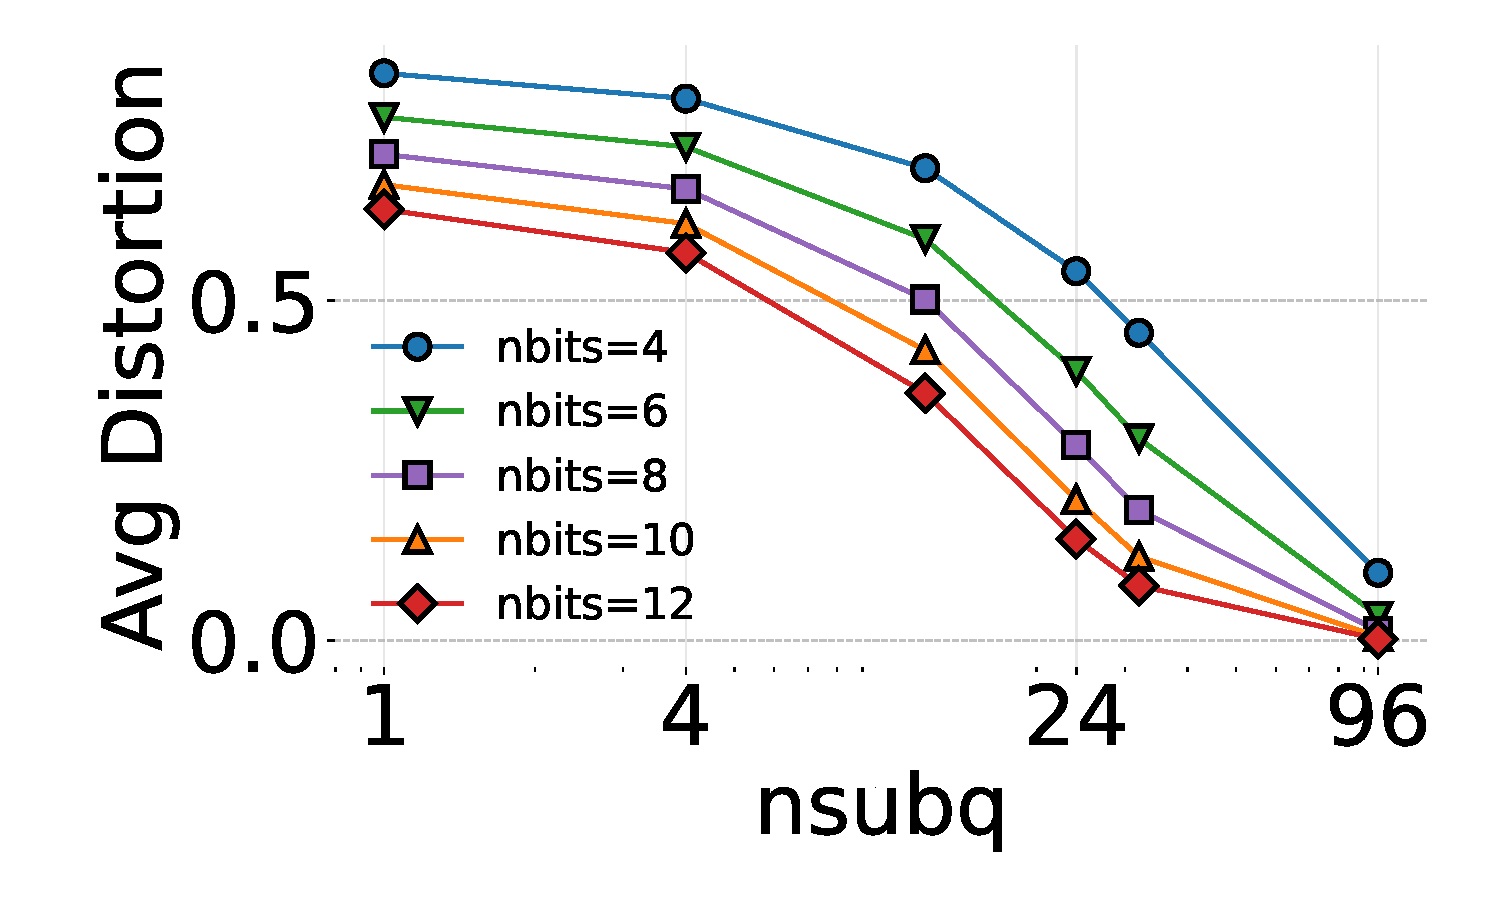
\includegraphics[width=\linewidth]{res/figures/pq_opq/distortion_error/distortionerror_pq_deep_nsubquantizers.pdf}
  % \caption{DEEP1M}
  % \label{fig:distortion-nsubq-deep}
\end{subfigure}\hfill
\begin{subfigure}[t]{0.19\textwidth}
  \centering
  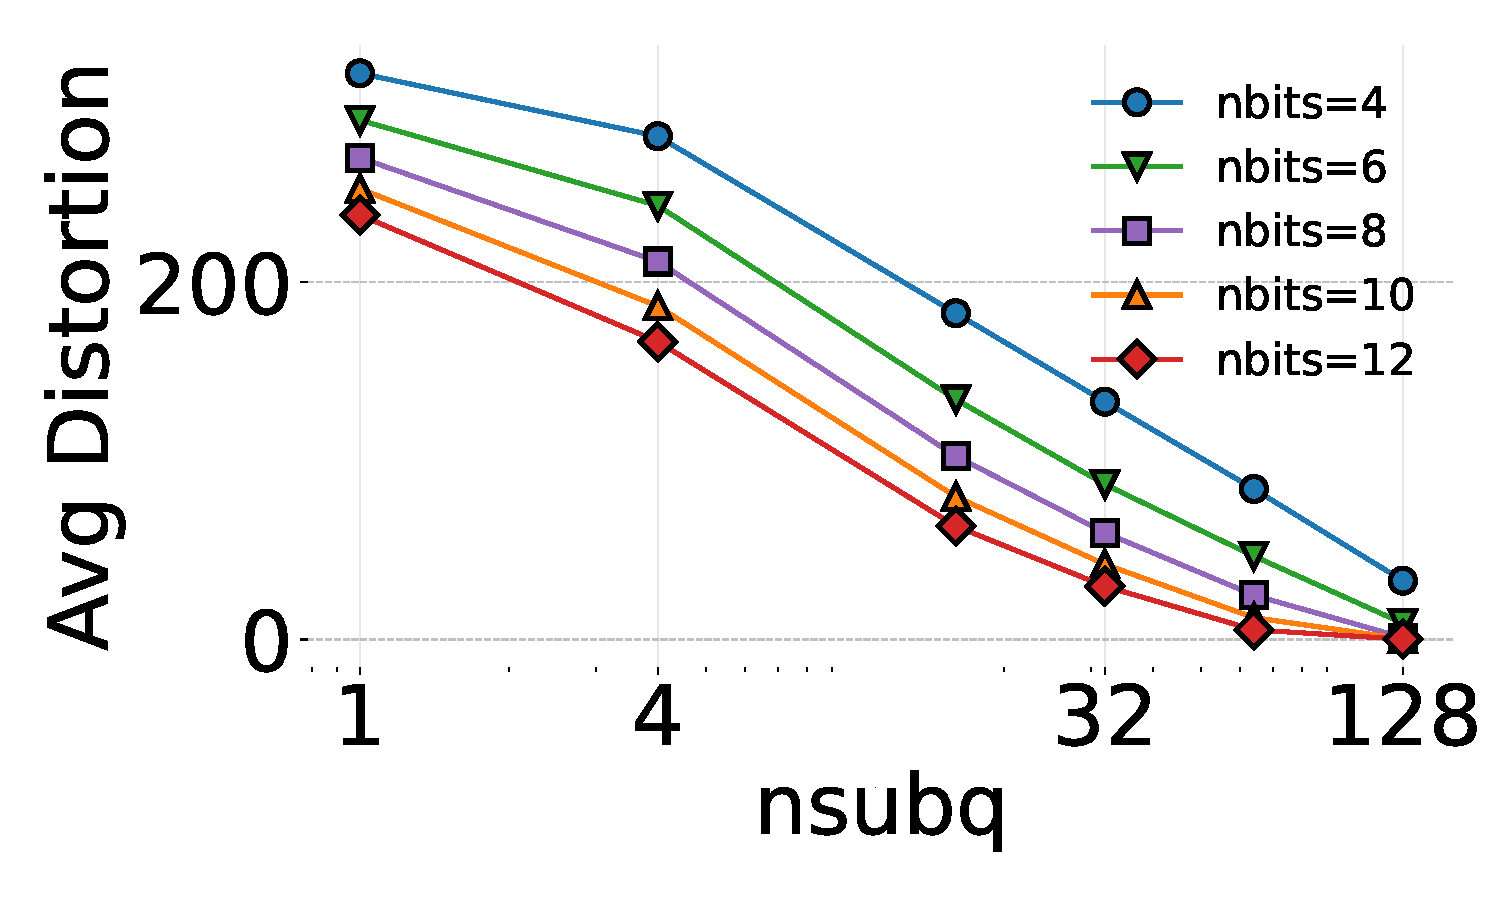
\includegraphics[width=\linewidth]{res/figures/pq_opq/distortion_error/distortionerror_pq_bigann_nsubquantizers.pdf}
  % \caption{SIFT1M}
  % \label{fig:distortion-nsubq-sift}
\end{subfigure}\hfill
\begin{subfigure}[t]{0.19\textwidth}
  \centering
  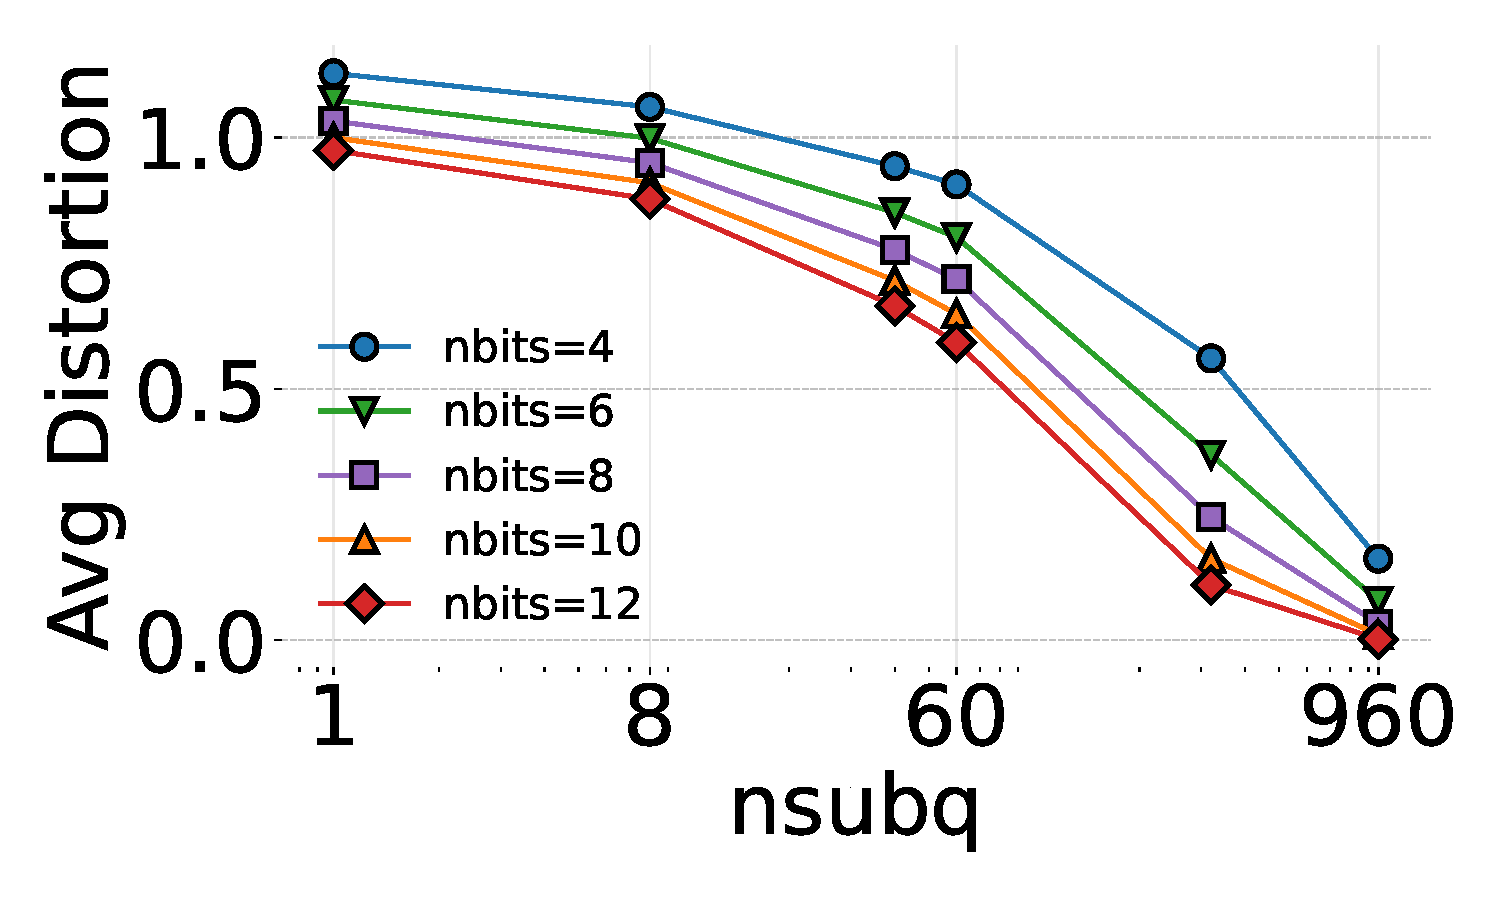
\includegraphics[width=\linewidth]{res/figures/pq_opq/distortion_error/distortionerror_pq_gist_nsubquantizers.pdf}
  % \caption{GIST1M}
  % \label{fig:distortion-nsubq-gist}
\end{subfigure}\hfill
\begin{subfigure}[t]{0.19\textwidth}
  \centering
  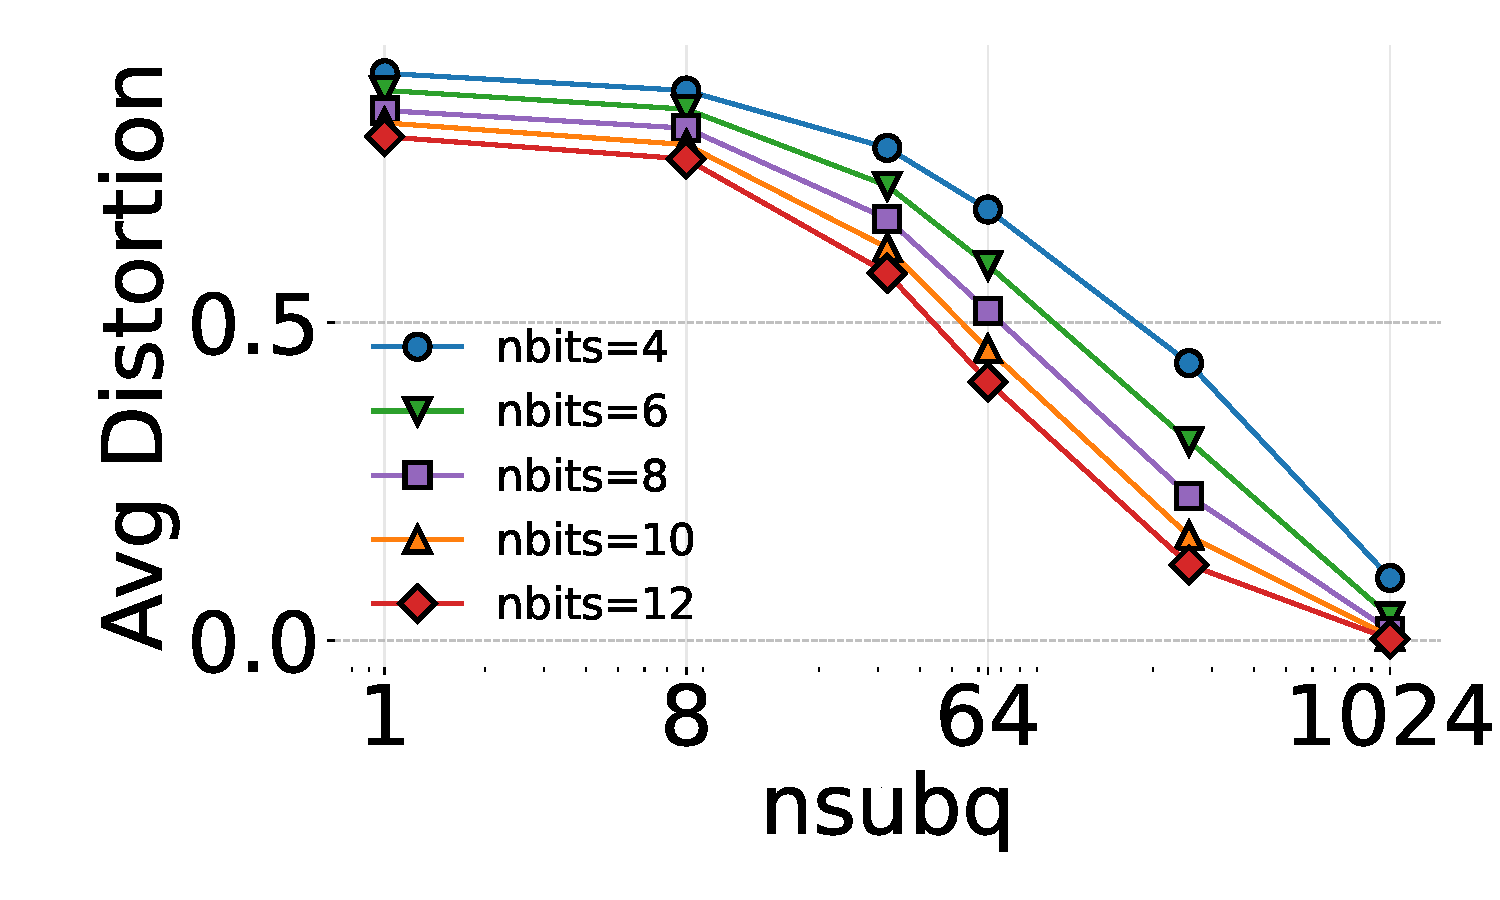
\includegraphics[width=\linewidth]{res/figures/pq_opq/distortion_error/distortionerror_pq_msmarco_nsubquantizers.pdf}
  % \caption{MSMARCO1M}
  % \label{fig:distortion-nsubq-msmarco}
\end{subfigure}\hfill
\begin{subfigure}[t]{0.19\textwidth}
  \centering
  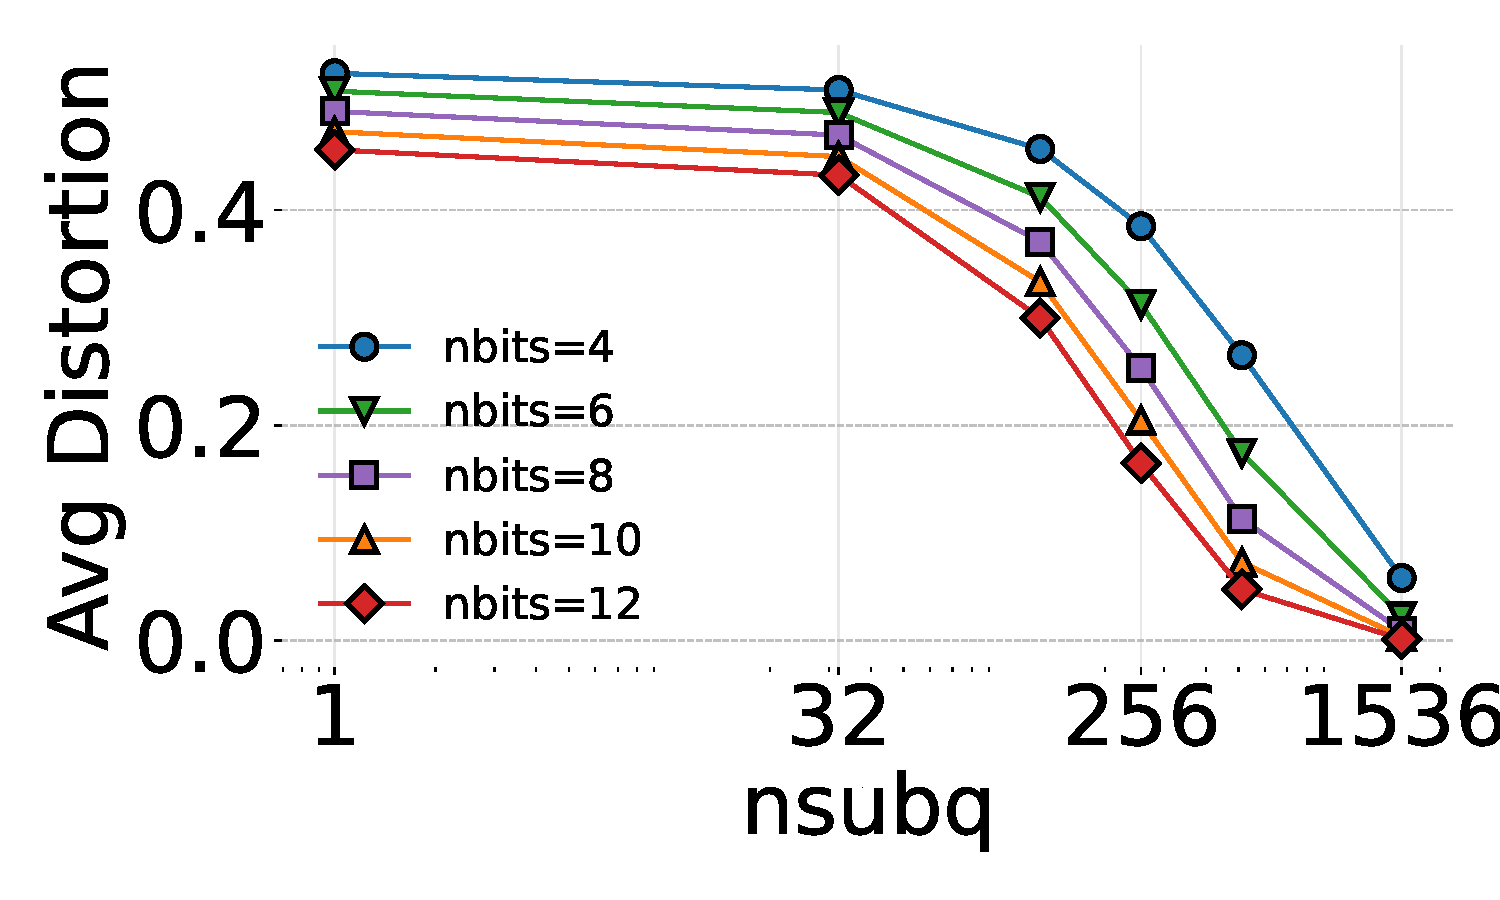
\includegraphics[width=\linewidth]{res/figures/pq_opq/distortion_error/distortionerror_pq_openai_nsubquantizers.pdf}
  % \caption{OpenAI-1536}
  % \label{fig:distortion-nsubq-openai}
\end{subfigure}


\par\medskip



\begin{subfigure}[t]{0.19\textwidth}
  \centering
  
\includegraphics[width=\linewidth]{res/figures/relerr_nbits/relerr_pq_deep_nbits.pdf}
  \label{fig:nbits-deep}
\end{subfigure}\hfill
\begin{subfigure}[t]{0.19\textwidth}
  \centering
  
\includegraphics[width=\linewidth]{res/figures/relerr_nbits/relerr_pq_bigann_nbits.pdf}
  \label{fig:nbits-sift}
\end{subfigure}\hfill
\begin{subfigure}[t]{0.19\textwidth}
  \centering
  
\includegraphics[width=\linewidth]{res/figures/relerr_nbits/relerr_pq_gist_nbits.pdf}
  \label{fig:nbits-gist}
\end{subfigure}\hfill
\begin{subfigure}[t]{0.19\textwidth}
  \centering
  
\includegraphics[width=\linewidth]{res/figures/relerr_nbits/relerr_pq_msmarco_nbits.pdf}
  \label{fig:nbits-msmarco}
\end{subfigure}\hfill
\begin{subfigure}[t]{0.19\textwidth}
  \centering
  
\includegraphics[width=\linewidth]{res/figures/relerr_nbits/relerr_pq_openai_nbits.pdf}
  \label{fig:nbits-openai}
\end{subfigure}


\par\medskip



\begin{subfigure}[t]{0.19\textwidth}
  \centering
  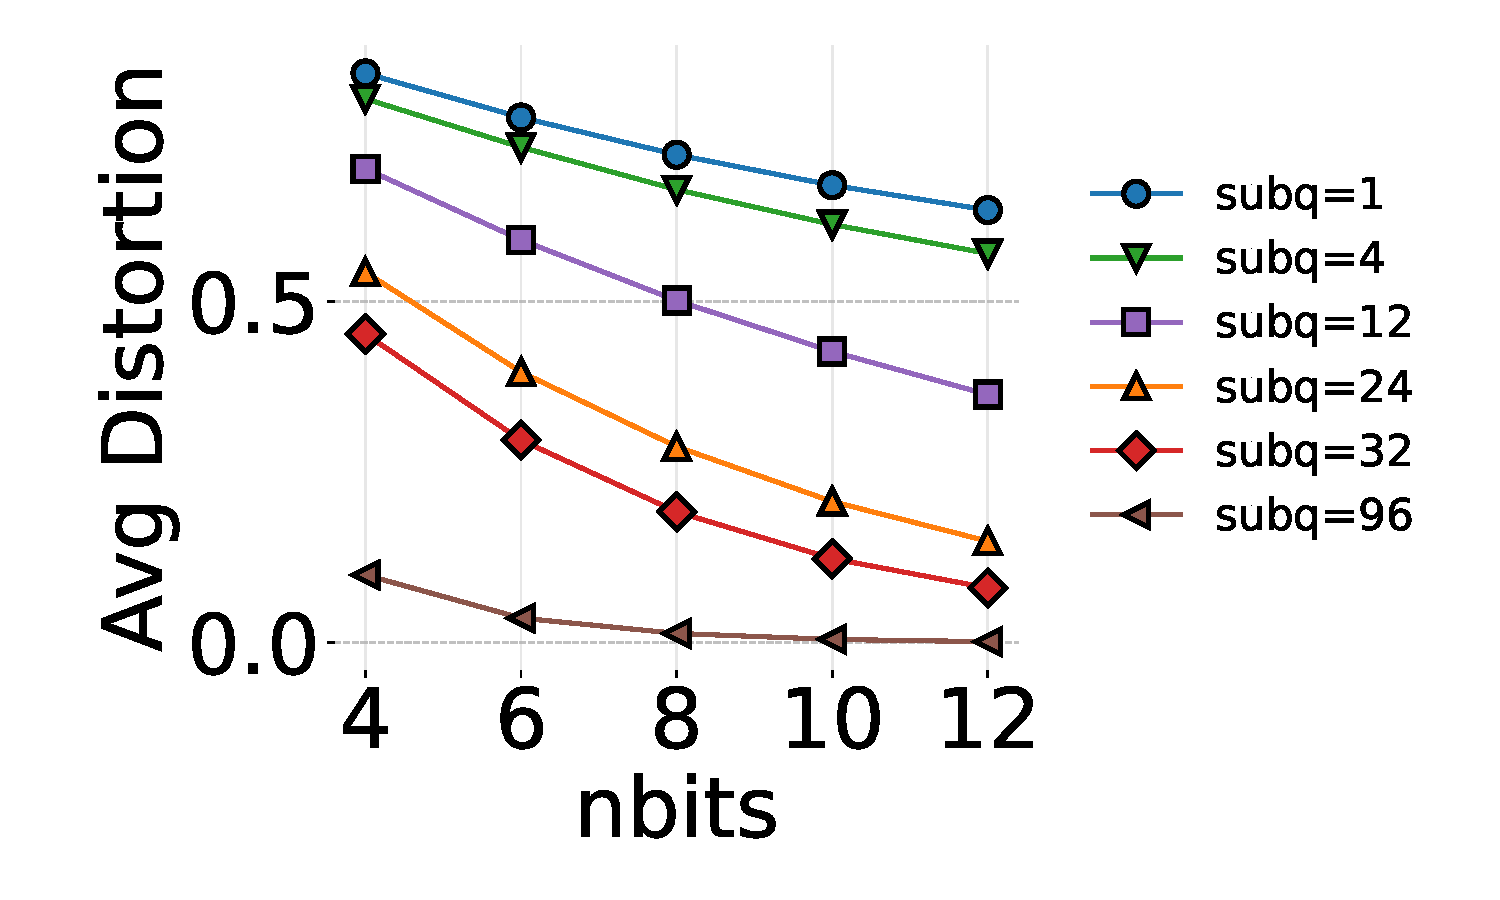
\includegraphics[width=\linewidth]{res/figures/pq_opq/distortion_error/distortionerror_pq_deep_nbits.pdf}
  \label{fig:distortion-nbits-deep}
\end{subfigure}\hfill
\begin{subfigure}[t]{0.19\textwidth}
  \centering
  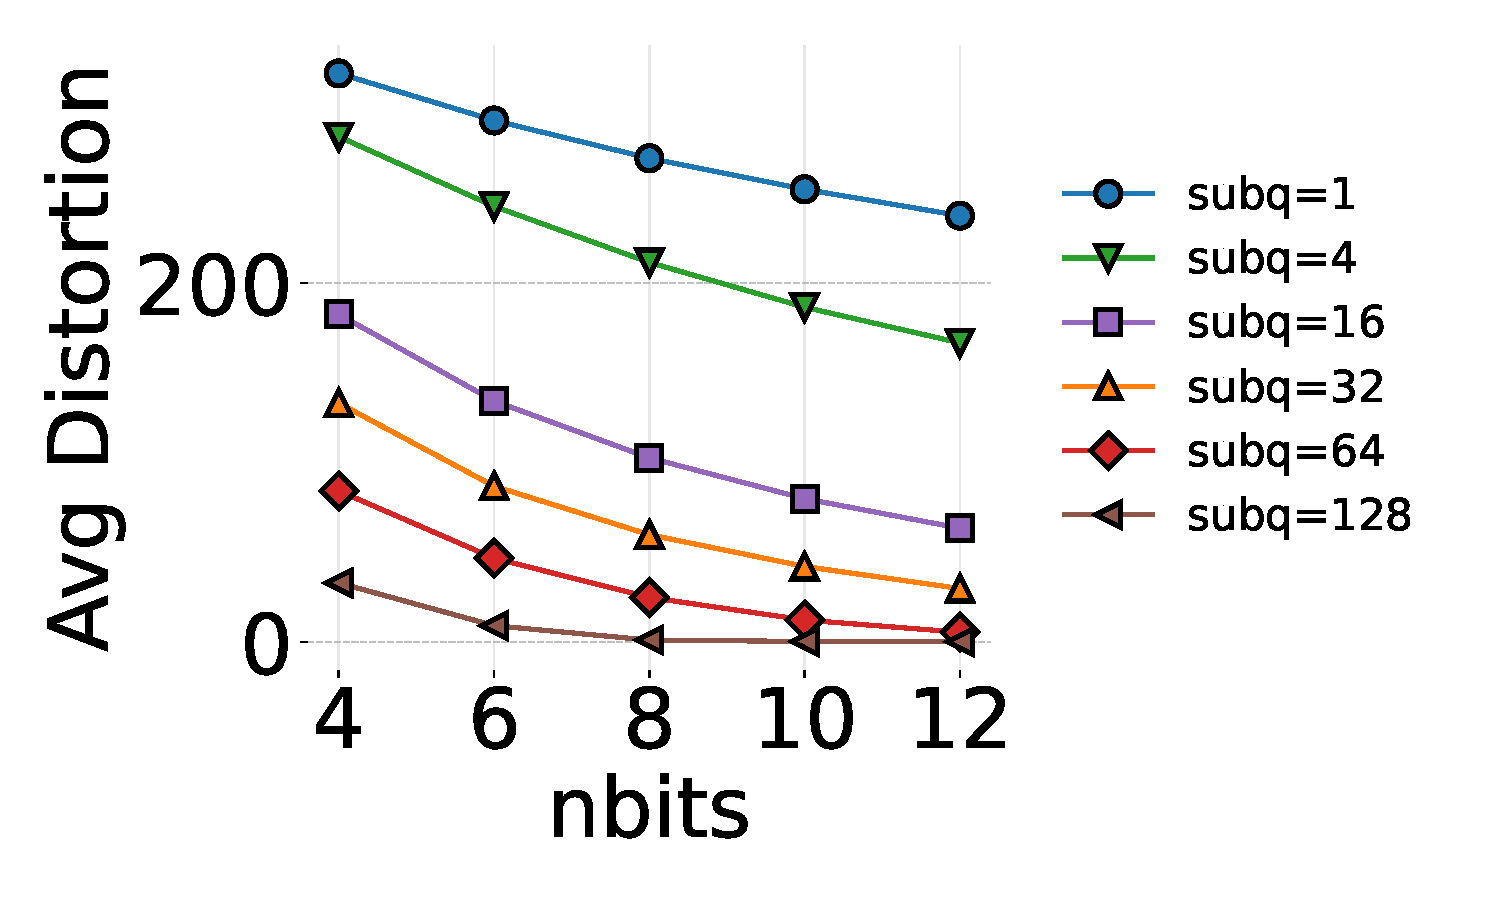
\includegraphics[width=\linewidth]{res/figures/pq_opq/distortion_error/distortionerror_pq_bigann_nbits.pdf}
  \label{fig:distortion-nbits-sift}
\end{subfigure}\hfill
\begin{subfigure}[t]{0.19\textwidth}
  \centering
  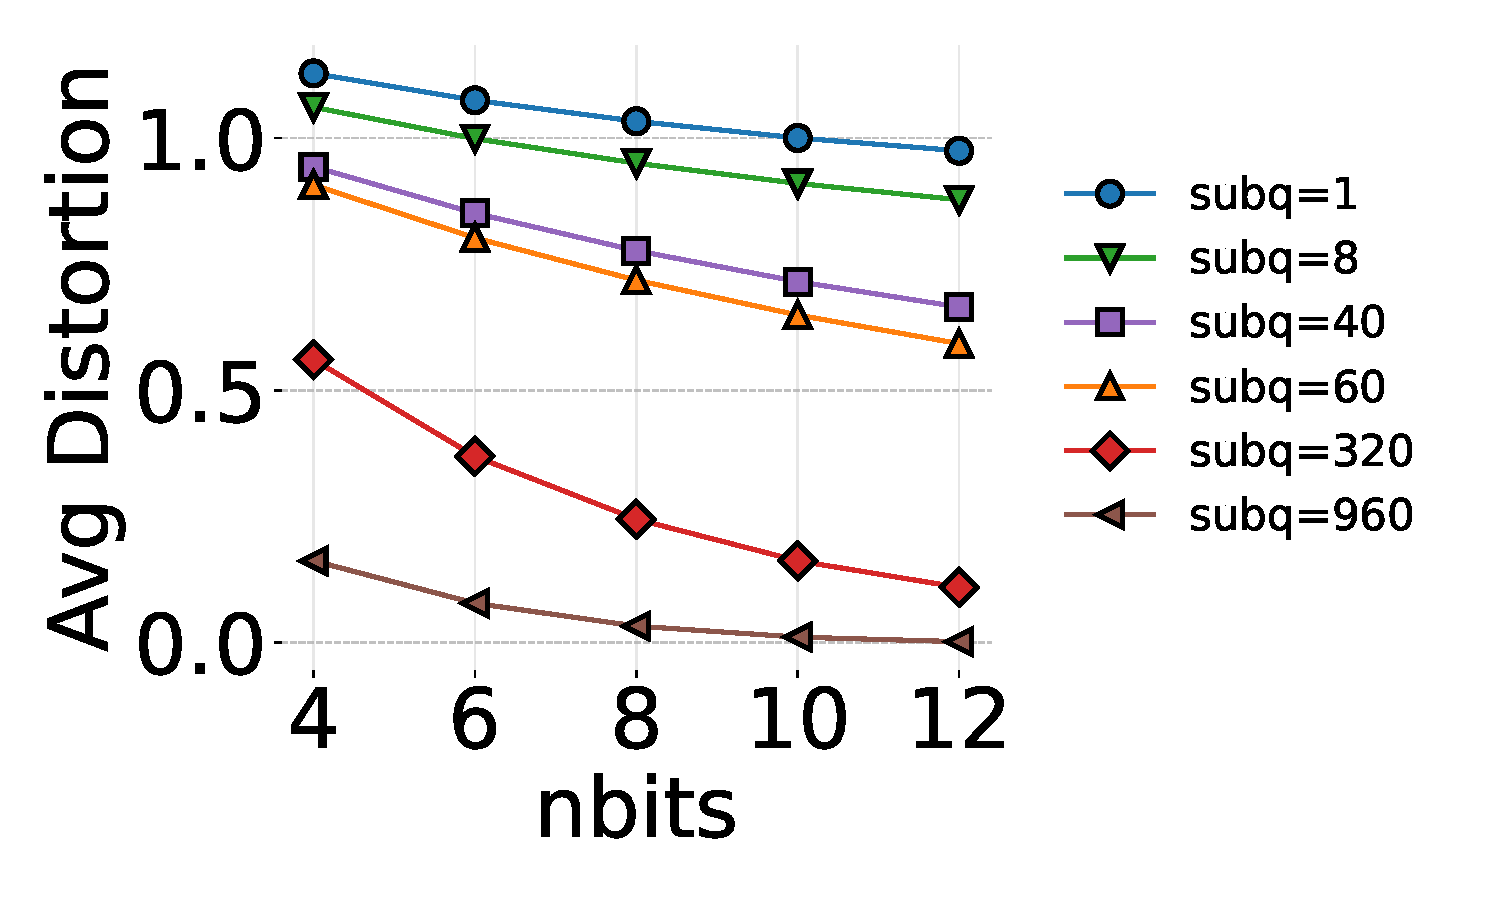
\includegraphics[width=\linewidth]{res/figures/pq_opq/distortion_error/distortionerror_pq_gist_nbits.pdf}
  \label{fig:distortion-nbits-gist}
\end{subfigure}\hfill
\begin{subfigure}[t]{0.19\textwidth}
  \centering
  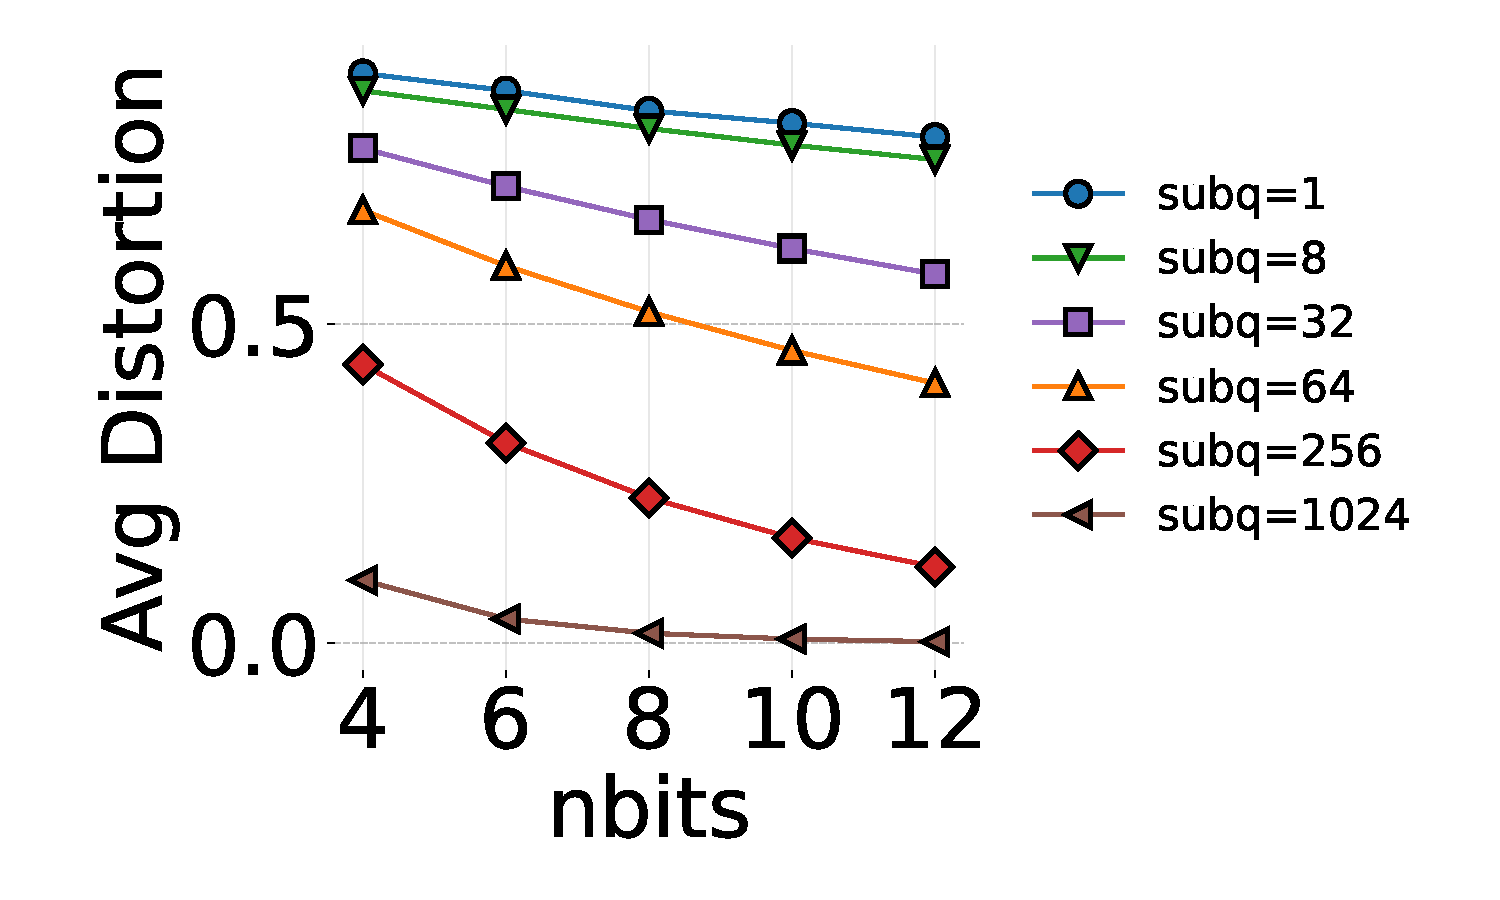
\includegraphics[width=\linewidth]{res/figures/pq_opq/distortion_error/distortionerror_pq_msmarco_nbits.pdf}
  \label{fig:distortion-nbits-msmarco}
\end{subfigure}\hfill
\begin{subfigure}[t]{0.19\textwidth}
  \centering
  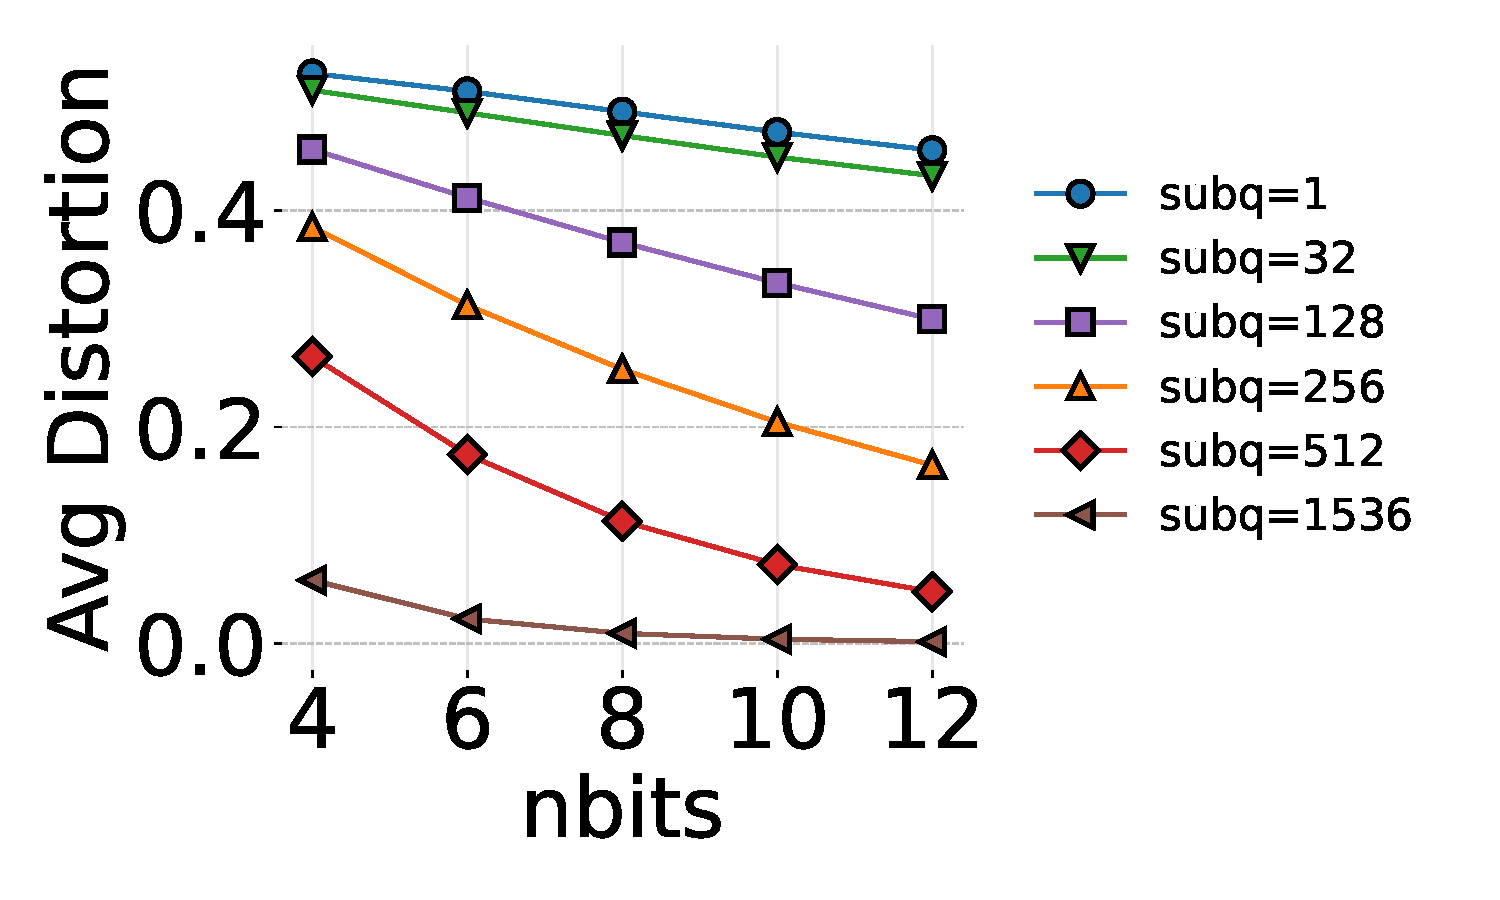
\includegraphics[width=\linewidth]{res/figures/pq_opq/distortion_error/distortionerror_pq_openai_nbits.pdf}
  \label{fig:distortion-nbits-openai}
\end{subfigure}


\par\medskip



\begin{subfigure}[t]{0.19\textwidth}
  \centering
  
\includegraphics[width=\linewidth]{res/figures/relerr_train_size/deep_PQ_train_size_vs_relerr.pdf}
  \label{fig:train_size-deep}
\end{subfigure}\hfill
\begin{subfigure}[t]{0.19\textwidth}
  \centering
  
\includegraphics[width=\linewidth]{res/figures/relerr_train_size/bigann_PQ_train_size_vs_relerr.pdf}
  \label{fig:train_size-sift}
\end{subfigure}\hfill
\begin{subfigure}[t]{0.19\textwidth}
  \centering
  
\includegraphics[width=\linewidth]{res/figures/relerr_train_size/gist_PQ_train_size_vs_relerr.pdf}
  \label{fig:train_size-gist}
\end{subfigure}\hfill
\begin{subfigure}[t]{0.19\textwidth}
  \centering
  
\includegraphics[width=\linewidth]{res/figures/relerr_train_size/msmarco_PQ_train_size_vs_relerr.pdf}
  \label{fig:train_size-msmarco}
\end{subfigure}\hfill
\begin{subfigure}[t]{0.19\textwidth}
  \centering
  
\includegraphics[width=\linewidth]{res/figures/relerr_train_size/openai_PQ_train_size_vs_relerr.pdf}
  \label{fig:train_size-openai}
\end{subfigure}

\par\medskip

\begin{subfigure}[t]{0.19\textwidth}
  \centering
  
\includegraphics[width=\linewidth]{res/figures/adc_vs_bits_per_vec/paper_adc_vs_bits_per_vector_deep.pdf}
  \label{fig:adc_vs_bpv-deep}
\end{subfigure}\hfill
\begin{subfigure}[t]{0.19\textwidth}
  \centering
  
\includegraphics[width=\linewidth]{res/figures/adc_vs_bits_per_vec/paper_adc_vs_bits_per_vector_bigann.pdf}
  \label{fig:adc_vs_bpv-sift}
\end{subfigure}\hfill
\begin{subfigure}[t]{0.19\textwidth}
  \centering
  
\includegraphics[width=\linewidth]{res/figures/adc_vs_bits_per_vec/paper_adc_vs_bits_per_vector_gist.pdf}
  \label{fig:adc_vs_bpv-gist}
\end{subfigure}\hfill
\begin{subfigure}[t]{0.19\textwidth}
  \centering
  
\includegraphics[width=\linewidth]{res/figures/adc_vs_bits_per_vec/paper_adc_vs_bits_per_vector_msmarco.pdf}
  \label{fig:adc_vs_bpv-msmarco}
\end{subfigure}\hfill
\begin{subfigure}[t]{0.19\textwidth}
  \centering
  
\includegraphics[width=\linewidth]{res/figures/adc_vs_bits_per_vec/paper_adc_vs_bits_per_vector_openai.pdf}
  \label{fig:adc_vs_bpv-openai}
\end{subfigure}

\par\medskip

\begin{subfigure}[t]{0.19\textwidth}
  \centering
  
\includegraphics[width=\linewidth]{res/figures/adc_vs_nbits/paper_adc_vs_nbits_by_M_deep.pdf}
  \label{fig:adc_vs_nbits-deep}
\end{subfigure}\hfill
\begin{subfigure}[t]{0.19\textwidth}
  \centering
  
\includegraphics[width=\linewidth]{res/figures/adc_vs_nbits/paper_adc_vs_nbits_by_M_bigann.pdf}
  \label{fig:adc_vs_nbits-sift}
\end{subfigure}\hfill
\begin{subfigure}[t]{0.19\textwidth}
  \centering
  
\includegraphics[width=\linewidth]{res/figures/adc_vs_nbits/paper_adc_vs_nbits_by_M_gist.pdf}
  \label{fig:adc_vs_nbits-gist}
\end{subfigure}\hfill
\begin{subfigure}[t]{0.19\textwidth}
  \centering
  
\includegraphics[width=\linewidth]{res/figures/adc_vs_nbits/paper_adc_vs_nbits_by_M_msmarco.pdf}
  \label{fig:adc_vs_nbits-msmarco}
\end{subfigure}\hfill
\begin{subfigure}[t]{0.19\textwidth}
  \centering
  
\includegraphics[width=\linewidth]{res/figures/adc_vs_nbits/paper_adc_vs_nbits_by_M_openai.pdf}
  \label{fig:adc_vs_nbits-openai}
\end{subfigure}


\par\medskip


\begin{subfigure}[t]{0.19\textwidth}
  \centering
  
\includegraphics[width=\linewidth]{res/figures/adc_vs_nsubq/paper_adc_vs_M_by_nbits_deep.pdf}
  \label{fig:adc_vs_M-deep}
\end{subfigure}\hfill
\begin{subfigure}[t]{0.19\textwidth}
  \centering
  
\includegraphics[width=\linewidth]{res/figures/adc_vs_nsubq/paper_adc_vs_M_by_nbits_bigann.pdf}
  \label{fig:adc_vs_M-sift}
\end{subfigure}\hfill
\begin{subfigure}[t]{0.19\textwidth}
  \centering
  
\includegraphics[width=\linewidth]{res/figures/adc_vs_nsubq/paper_adc_vs_M_by_nbits_gist.pdf}
  \label{fig:adc_vs_M-gist}
\end{subfigure}\hfill
\begin{subfigure}[t]{0.19\textwidth}
  \centering
  
\includegraphics[width=\linewidth]{res/figures/adc_vs_nsubq/paper_adc_vs_M_by_nbits_msmarco.pdf}
  \label{fig:adc_vs_M-msmarco}
\end{subfigure}\hfill
\begin{subfigure}[t]{0.19\textwidth}
  \centering
  
\includegraphics[width=\linewidth]{res/figures/adc_vs_nsubq/paper_adc_vs_M_by_nbits_openai.pdf}
  \label{fig:adc_vs_M-openai}
\end{subfigure}


\par\medskip


\begin{subfigure}[t]{0.19\textwidth}
  \centering
  
\includegraphics[width=\linewidth]{res/figures/pareto_bpv/paper_relerr_vs_adc_by_bpv_deep.pdf}
  \caption{DEEP1M}
  \label{fig:pareto_bpv-deep}
\end{subfigure}\hfill
\begin{subfigure}[t]{0.19\textwidth}
  \centering
  
\includegraphics[width=\linewidth]{res/figures/pareto_bpv/paper_relerr_vs_adc_by_bpv_bigann.pdf}
  \caption{SIFT1M}
  \label{fig:pareto_bpv-sift}
\end{subfigure}\hfill
\begin{subfigure}[t]{0.19\textwidth}
  \centering
  
\includegraphics[width=\linewidth]{res/figures/pareto_bpv/paper_relerr_vs_adc_by_bpv_gist.pdf}
  \caption{GIST1M}
  \label{fig:pareto_bpv-gist}
\end{subfigure}\hfill
\begin{subfigure}[t]{0.19\textwidth}
  \centering
  
\includegraphics[width=\linewidth]{res/figures/pareto_bpv/paper_relerr_vs_adc_by_bpv_msmarco.pdf}
  \caption{MSMARCO1M}
  \label{fig:pareto_bpv-msmarco}
\end{subfigure}\hfill
\begin{subfigure}[t]{0.19\textwidth}
  \centering
  
\includegraphics[width=\linewidth]{res/figures/pareto_bpv/paper_relerr_vs_adc_by_bpv_openai.pdf}
  \caption{OpenAI-1536}
  \label{fig:pareto_bpv-openai}
\end{subfigure}




\caption{PQ's Hyper-parameters influence on relative error and per-pair distance computation time}
\label{fig:pq_hp_inf}
\end{figure*}

\subsection{Baseline Comparison}
\subsubsection{OPQ improvement analysis}
OPQ improves upon PQ by learning a rotation matrix that is applied to the data before the quantization step. 
This rotation aims to rearrange the vector dimensions such that relevant dimensions are grouped within the same subspaces during the subquantizer partitioning. 
By preserving relevant dimensions within subspaces, the clustering process becomes more effective, leading to improved compression quality and more accurate distance approximations.

In the first row of Figure~\ref{fig:opq_rot_improvement}, we illustrate the improvement in relative error achieved by OPQ over PQ, averaged across the different values of \textit{nsubq} and \textit{nbits}. 
The improvement is shown as a function of the percentage of the training data used to learn the rotation matrix $R$.
In the second row of Figure~\ref{fig:opq_rot_improvement}, we observe that the most significant improvement is already obtained when using only $10\%$ of the available training data to learn the rotation matrix. 
This introduces only a small additional training overhead while still yielding a clear improvement in approximation accuracy.still providing a clear improvement in approximation accuracy.

Overall, these observations confirm that OPQ provides a reliable improvement over PQ, as it enhances the effectiveness of the subspace partitioning without requiring large additional training costs.


% Requires in the preamble:
% \usepackage{subcaption}
\begin{figure*}[t]
\centering

\begin{subfigure}[t]{0.19\textwidth}
  \centering
  
\includegraphics[width=\linewidth]{res/figures/relerr_opq_vs_pq/opq_vs_pq_rot_pct_relerrormean_deep_M1-96_nbits4-12.pdf}
  \label{fig:opq_vs_pq_rot-deep}
\end{subfigure}\hfill
\begin{subfigure}[t]{0.19\textwidth}
  \centering
  \includegraphics[width=\linewidth]{}
  \label{fig:opq_vs_pq_rot-sift}
\end{subfigure}\hfill
\begin{subfigure}[t]{0.19\textwidth}
  \centering
  
\includegraphics[width=\linewidth]{res/figures/relerr_opq_vs_pq/opq_vs_pq_rot_pct_relerrormean_gist_M1-960_nbits4-12.pdf}
  \label{fig:opq_vs_pq_rot-gist}
\end{subfigure}\hfill
\begin{subfigure}[t]{0.19\textwidth}
  \centering
  
\includegraphics[width=\linewidth]{res/figures/relerr_opq_vs_pq/opq_vs_pq_rot_pct_relerrormean_msmarco_M1-1024_nbits4-12.pdf}
  \label{fig:opq_vs_pq_rot-msmarco}
\end{subfigure}\hfill
\begin{subfigure}[t]{0.19\textwidth}
  \centering
  \includegraphics[width=\linewidth]{}
  \label{fig:opq_vs_pq_rot-openai}
\end{subfigure}


\par\medskip


\begin{subfigure}[t]{0.19\textwidth}
  \centering
  
\includegraphics[width=\linewidth]{res/figures/relerr_opq_vs_pq/opq_vs_pq_train_time_rot_pct_deep_M1-96_nbits4-12.pdf}
  \caption{DEEP1M}
  \label{fig:opq_vs_pq_train_time-deep}
\end{subfigure}\hfill
\begin{subfigure}[t]{0.19\textwidth}
  \centering
  \includegraphics[width=\linewidth]{}
  \caption{SIFT1M}
  \label{fig:opq_vs_pq_train_time-sift}
\end{subfigure}\hfill
\begin{subfigure}[t]{0.19\textwidth}
  \centering
  
\includegraphics[width=\linewidth]{res/figures/relerr_opq_vs_pq/opq_vs_pq_train_time_rot_pct_gist_M1-960_nbits4-12.pdf}
  \caption{GIST1M}
  \label{fig:opq_vs_pq_train_time-gist}
\end{subfigure}\hfill
\begin{subfigure}[t]{0.19\textwidth}
  \centering
  
\includegraphics[width=\linewidth]{res/figures/relerr_opq_vs_pq/opq_vs_pq_train_time_rot_pct_msmarco_M1-1024_nbits4-12.pdf}
  \caption{MSMARCO1M}
  \label{fig:opq_vs_pq_train_time-msmarco}
\end{subfigure}\hfill
\begin{subfigure}[t]{0.19\textwidth}
  \centering
  \includegraphics[width=\linewidth]{}
  \caption{OpenAI-1536}
  \label{fig:opq_vs_pq_train_time-openai}
\end{subfigure}



\caption{OPQ's rotation learning influence on relative error and training time}
\label{fig:opq_rot_improvement}
\end{figure*}


% Requires:
% \usepackage{subcaption}
% \usepackage{graphicx}

\newcommand{\lsqppplot}[2]{%
\begin{subfigure}[t]{0.19\textwidth}
  \centering
  \includegraphics[width=\linewidth]{res/figures/lsqpp/#1_lsqpp_#2.pdf}
\end{subfigure}%
}

\newcommand{\lsqppplotcaption}[3]{%
\begin{subfigure}[t]{0.19\textwidth}
  \centering
  \includegraphics[width=\linewidth]{res/figures/lsqpp/#1_lsqpp_#2.pdf}
  \caption{#3}
  \label{fig:lsqpp-#1-#2}
\end{subfigure}%
}

\begin{figure*}[t]
\centering

% Row 1: Relative error vs number of codebooks / M
\lsqppplot{avg_relerr_vs_M_with_config_legend}{bigann}\hfill
\lsqppplot{avg_relerr_vs_M_with_config_legend}{deep}\hfill
\lsqppplot{avg_relerr_vs_M_with_config_legend}{gist}\hfill
\lsqppplot{avg_relerr_vs_M_with_config_legend}{msmarco}\hfill
\lsqppplot{avg_relerr_vs_M_with_config_legend}{openai}

\par\medskip

% Row 2: Relative error vs nbits
\lsqppplot{avg_relerr_vs_nbits_with_config_legend}{bigann}\hfill
\lsqppplot{avg_relerr_vs_nbits_with_config_legend}{deep}\hfill
\lsqppplot{avg_relerr_vs_nbits_with_config_legend}{gist}\hfill
\lsqppplot{avg_relerr_vs_nbits_with_config_legend}{msmarco}\hfill
\lsqppplot{avg_relerr_vs_nbits_with_config_legend}{openai}

\par\medskip

% Row 3: Relative error vs training size, grouped by M
\lsqppplot{avg_relerr_vs_train_size_legend_M}{bigann}\hfill
\lsqppplot{avg_relerr_vs_train_size_legend_M}{deep}\hfill
\lsqppplot{avg_relerr_vs_train_size_legend_M}{gist}\hfill
\lsqppplot{avg_relerr_vs_train_size_legend_M}{msmarco}\hfill
\lsqppplot{avg_relerr_vs_train_size_legend_M}{openai}

\par\medskip

% Row 4: Relative error vs training size, with full configuration legend
\lsqppplot{avg_relerr_vs_train_size_with_config_legend}{bigann}\hfill
\lsqppplot{avg_relerr_vs_train_size_with_config_legend}{deep}\hfill
\lsqppplot{avg_relerr_vs_train_size_with_config_legend}{gist}\hfill
\lsqppplot{avg_relerr_vs_train_size_with_config_legend}{msmarco}\hfill
\lsqppplot{avg_relerr_vs_train_size_with_config_legend}{openai}

\par\medskip

% Row 5: ADC time vs M
\lsqppplot{adc_time_vs_M_with_config_legend}{bigann}\hfill
\lsqppplot{adc_time_vs_M_with_config_legend}{deep}\hfill
\lsqppplot{adc_time_vs_M_with_config_legend}{gist}\hfill
\lsqppplot{adc_time_vs_M_with_config_legend}{msmarco}\hfill
\lsqppplot{adc_time_vs_M_with_config_legend}{openai}

\par\medskip

% Row 6: ADC time vs nbits
\lsqppplot{adc_time_vs_nbits_with_config_legend}{bigann}\hfill
\lsqppplot{adc_time_vs_nbits_with_config_legend}{deep}\hfill
\lsqppplot{adc_time_vs_nbits_with_config_legend}{gist}\hfill
\lsqppplot{adc_time_vs_nbits_with_config_legend}{msmarco}\hfill
\lsqppplot{adc_time_vs_nbits_with_config_legend}{openai}

\par\medskip

% Row 7: Pareto plots, with dataset captions
\lsqppplotcaption{pareto_relerr_vs_adc_time}{bigann}{SIFT1M}\hfill
\lsqppplotcaption{pareto_relerr_vs_adc_time}{deep}{DEEP1M}\hfill
\lsqppplotcaption{pareto_relerr_vs_adc_time}{gist}{GIST1M}\hfill
\lsqppplotcaption{pareto_relerr_vs_adc_time}{msmarco}{MSMARCO1M}\hfill
\lsqppplotcaption{pareto_relerr_vs_adc_time}{openai}{OpenAI-1536}

\caption{LSQ++ hyperparameter influence on relative error and per-pair approximate distance computation time. Rows report the effect of the number of codebooks $M$, number of bits per codebook, training size, and the resulting relative-error--time Pareto frontier across datasets.}
\label{fig:lsqpp_hp_inf}
\end{figure*}


% \newcommand{\vaqplot}[2]{%
% \begin{subfigure}[t]{0.19\textwidth}
%   \centering
%   \includegraphics[width=\linewidth]{res/figures/vaq/#1_vaq_#2.pdf}
% \end{subfigure}%
% }

% \newcommand{\vaqplotcaption}[3]{%
% \begin{subfigure}[t]{0.19\textwidth}
%   \centering
%   \includegraphics[width=\linewidth]{res/figures/vaq/#1_vaq_#2.pdf}
%   \caption{#3}
%   \label{fig:vaq-#1-#2}
% \end{subfigure}%
% }

% \begin{figure*}[t]
% \centering

% % Row 1: Relative error vs bits per vector, varying max_bits
% \vaqplot{avg_relerr_vs_bits_per_vector_legend_max_bits}{bigann}\hfill
% \vaqplot{avg_relerr_vs_bits_per_vector_legend_max_bits}{deep}\hfill
% \vaqplot{avg_relerr_vs_bits_per_vector_legend_max_bits}{gist}\hfill
% \vaqplot{avg_relerr_vs_bits_per_vector_legend_max_bits}{msmarco}\hfill
% \vaqplot{avg_relerr_vs_bits_per_vector_legend_max_bits}{openai}

% \par\medskip

% % Row 2: Relative error vs bits per vector, varying min_bits
% \vaqplot{avg_relerr_vs_bits_per_vector_legend_min_bits}{bigann}\hfill
% \vaqplot{avg_relerr_vs_bits_per_vector_legend_min_bits}{deep}\hfill
% \vaqplot{avg_relerr_vs_bits_per_vector_legend_min_bits}{gist}\hfill
% \vaqplot{avg_relerr_vs_bits_per_vector_legend_min_bits}{msmarco}\hfill
% \vaqplot{avg_relerr_vs_bits_per_vector_legend_min_bits}{openai}

% \par\medskip

% % Row 3: Relative error vs max_bits, grouped by min_bits
% \vaqplot{avg_relerr_vs_max_bits_legend_min_bits}{bigann}\hfill
% \vaqplot{avg_relerr_vs_max_bits_legend_min_bits}{deep}\hfill
% \vaqplot{avg_relerr_vs_max_bits_legend_min_bits}{gist}\hfill
% \vaqplot{avg_relerr_vs_max_bits_legend_min_bits}{msmarco}\hfill
% \vaqplot{avg_relerr_vs_max_bits_legend_min_bits}{openai}

% \par\medskip

% % Row 4: Relative error vs min_bits, grouped by max_bits
% \vaqplot{avg_relerr_vs_min_bits_legend_max_bits}{bigann}\hfill
% \vaqplot{avg_relerr_vs_min_bits_legend_max_bits}{deep}\hfill
% \vaqplot{avg_relerr_vs_min_bits_legend_max_bits}{gist}\hfill
% \vaqplot{avg_relerr_vs_min_bits_legend_max_bits}{msmarco}\hfill
% \vaqplot{avg_relerr_vs_min_bits_legend_max_bits}{openai}

% \par\medskip

% % Row 5: ADC time vs max_bits, grouped by min_bits
% \vaqplot{adc_time_vs_max_bits_legend_min_bits}{bigann}\hfill
% \vaqplot{adc_time_vs_max_bits_legend_min_bits}{deep}\hfill
% \vaqplot{adc_time_vs_max_bits_legend_min_bits}{gist}\hfill
% \vaqplot{adc_time_vs_max_bits_legend_min_bits}{msmarco}\hfill
% \vaqplot{adc_time_vs_max_bits_legend_min_bits}{openai}

% \par\medskip

% % Row 6: ADC time vs min_bits, grouped by max_bits
% \vaqplot{adc_time_vs_min_bits_legend_max_bits}{bigann}\hfill
% \vaqplot{adc_time_vs_min_bits_legend_max_bits}{deep}\hfill
% \vaqplot{adc_time_vs_min_bits_legend_max_bits}{gist}\hfill
% \vaqplot{adc_time_vs_min_bits_legend_max_bits}{msmarco}\hfill
% \vaqplot{adc_time_vs_min_bits_legend_max_bits}{openai}

% \par\medskip

% % Row 7: Pareto plots, with dataset captions
% \vaqplotcaption{pareto_relerr_vs_adc_time}{bigann}{SIFT1M}\hfill
% \vaqplotcaption{pareto_relerr_vs_adc_time}{deep}{DEEP1M}\hfill
% \vaqplotcaption{pareto_relerr_vs_adc_time}{gist}{GIST1M}\hfill
% \vaqplotcaption{pareto_relerr_vs_adc_time}{msmarco}{MSMARCO1M}\hfill
% \vaqplotcaption{pareto_relerr_vs_adc_time}{openai}{OpenAI-1536}

% \caption{VAQ hyperparameter influence on relative error and per-pair approximate distance computation time. Rows report the effect of the total bit budget, minimum and maximum bits per subspace, and the resulting relative-error--time Pareto frontier across datasets.}
% \label{fig:vaq_hp_inf}
% \end{figure*}


% Requires:
% \usepackage{subcaption}
% \usepackage{graphicx}

\newcommand{\rabitqplot}[2]{%
\begin{subfigure}[t]{0.19\textwidth}
  \centering
  \includegraphics[width=\linewidth]{res/figures/rabitq/#1_rabitq_saqfair_#2.pdf}
\end{subfigure}%
}

\newcommand{\rabitqplotcaption}[3]{%
\begin{subfigure}[t]{0.19\textwidth}
  \centering
  \includegraphics[width=\linewidth]{res/figures/rabitq/#1_rabitq_saqfair_#2.pdf}
  \caption{#3}
  \label{fig:rabitq-#1-#2}
\end{subfigure}%
}

\begin{figure*}[t]
\centering

% Row 1: Relative error vs bits per vector
\rabitqplot{relerr_vs_bits_per_vector}{bigann}\hfill
\rabitqplot{relerr_vs_bits_per_vector}{deep}\hfill
\rabitqplot{relerr_vs_bits_per_vector}{gist}\hfill
\rabitqplot{relerr_vs_bits_per_vector}{msmarco}\hfill
\rabitqplot{relerr_vs_bits_per_vector}{openai}

\par\medskip

% Row 2: Relative error vs nbits
\rabitqplot{relerr_vs_nbits}{bigann}\hfill
\rabitqplot{relerr_vs_nbits}{deep}\hfill
\rabitqplot{relerr_vs_nbits}{gist}\hfill
\rabitqplot{relerr_vs_nbits}{msmarco}\hfill
\rabitqplot{relerr_vs_nbits}{openai}

\par\medskip

% Row 3: ADC time vs bits per vector
\rabitqplot{adc_time_vs_bits_per_vector}{bigann}\hfill
\rabitqplot{adc_time_vs_bits_per_vector}{deep}\hfill
\rabitqplot{adc_time_vs_bits_per_vector}{gist}\hfill
\rabitqplot{adc_time_vs_bits_per_vector}{msmarco}\hfill
\rabitqplot{adc_time_vs_bits_per_vector}{openai}

\par\medskip

% Row 4: ADC time vs bits per dimension / nbits
\rabitqplot{adc_time_vs_nbits}{bigann}\hfill
\rabitqplot{adc_time_vs_nbits}{deep}\hfill
\rabitqplot{adc_time_vs_nbits}{gist}\hfill
\rabitqplot{adc_time_vs_nbits}{msmarco}\hfill
\rabitqplot{adc_time_vs_nbits}{openai}

\par\medskip

% Row 5: Encoding time vs bits per vector
\rabitqplot{encoding_time_vs_bits_per_vector}{bigann}\hfill
\rabitqplot{encoding_time_vs_bits_per_vector}{deep}\hfill
\rabitqplot{encoding_time_vs_bits_per_vector}{gist}\hfill
\rabitqplot{encoding_time_vs_bits_per_vector}{msmarco}\hfill
\rabitqplot{encoding_time_vs_bits_per_vector}{openai}

\par\medskip

% Row 6: Encoding time vs bits per dimension / nbits, with dataset captions
\rabitqplotcaption{encoding_time_vs_nbits}{bigann}{SIFT1M}\hfill
\rabitqplotcaption{encoding_time_vs_nbits}{deep}{DEEP1M}\hfill
\rabitqplotcaption{encoding_time_vs_nbits}{gist}{GIST1M}\hfill
\rabitqplotcaption{encoding_time_vs_nbits}{msmarco}{MSMARCO1M}\hfill
\rabitqplotcaption{encoding_time_vs_nbits}{openai}{OpenAI-1536}

\caption{RaBitQ hyperparameter influence on relative error, per-pair approximate distance computation time, and encoding time. Rows report the effect of bits per vector and bits per dimension on relative error, ADC time, and encoding time across datasets.}
\label{fig:rabitq_hp_inf}
\end{figure*}


% Requires:
% \usepackage{subcaption}
% \usepackage{graphicx}

\newcommand{\saqplot}[2]{%
\begin{subfigure}[t]{0.19\textwidth}
  \centering
  \includegraphics[width=\linewidth]{res/figures/saq/#1_saq_#2.pdf}
\end{subfigure}%
}

\newcommand{\saqplotcaption}[3]{%
\begin{subfigure}[t]{0.19\textwidth}
  \centering
  \includegraphics[width=\linewidth]{res/figures/saq/#1_saq_#2.pdf}
  \caption{#3}
  \label{fig:saq-#1-#2}
\end{subfigure}%
}

\begin{figure*}[t]
\centering

% Row 1: Relative error vs bits per vector
\saqplot{avg_relerr_vs_bits_per_vector}{bigann}\hfill
\saqplot{avg_relerr_vs_bits_per_vector}{deep}\hfill
\saqplot{avg_relerr_vs_bits_per_vector}{gist}\hfill
\saqplot{avg_relerr_vs_bits_per_vector}{msmarco}\hfill
\saqplot{avg_relerr_vs_bits_per_vector}{openai}

\par\medskip

% Row 2: Relative error vs bits per dimension / nbits
\saqplot{avg_relerr_vs_nbits}{bigann}\hfill
\saqplot{avg_relerr_vs_nbits}{deep}\hfill
\saqplot{avg_relerr_vs_nbits}{gist}\hfill
\saqplot{avg_relerr_vs_nbits}{msmarco}\hfill
\saqplot{avg_relerr_vs_nbits}{openai}

\par\medskip

% Row 3: ADC time vs bits per vector
\saqplot{adc_time_vs_bits_per_vector}{bigann}\hfill
\saqplot{adc_time_vs_bits_per_vector}{deep}\hfill
\saqplot{adc_time_vs_bits_per_vector}{gist}\hfill
\saqplot{adc_time_vs_bits_per_vector}{msmarco}\hfill
\saqplot{adc_time_vs_bits_per_vector}{openai}

\par\medskip

% Row 4: ADC time vs bits per dimension / nbits
\saqplot{adc_time_vs_nbits}{bigann}\hfill
\saqplot{adc_time_vs_nbits}{deep}\hfill
\saqplot{adc_time_vs_nbits}{gist}\hfill
\saqplot{adc_time_vs_nbits}{msmarco}\hfill
\saqplot{adc_time_vs_nbits}{openai}

\par\medskip

% Row 5: Encoding time vs bits per vector
\saqplot{encoding_time_vs_bits_per_vector}{bigann}\hfill
\saqplot{encoding_time_vs_bits_per_vector}{deep}\hfill
\saqplot{encoding_time_vs_bits_per_vector}{gist}\hfill
\saqplot{encoding_time_vs_bits_per_vector}{msmarco}\hfill
\saqplot{encoding_time_vs_bits_per_vector}{openai}

\par\medskip

% Row 6: Encoding time vs bits per dimension / nbits, with dataset captions
\saqplotcaption{encoding_time_vs_nbits}{bigann}{SIFT1M}\hfill
\saqplotcaption{encoding_time_vs_nbits}{deep}{DEEP1M}\hfill
\saqplotcaption{encoding_time_vs_nbits}{gist}{GIST1M}\hfill
\saqplotcaption{encoding_time_vs_nbits}{msmarco}{MSMARCO1M}\hfill
\saqplotcaption{encoding_time_vs_nbits}{openai}{OpenAI-1536}

\caption{SAQ hyperparameter influence on relative error, per-pair approximate distance computation time, and encoding time. Rows report the effect of bits per vector and bits per dimension on relative error, ADC time, and encoding time across datasets.}
\label{fig:saq_hp_inf}
\end{figure*}



\newcommand{\bpvcompplotcaption}[2]{%
\begin{subfigure}[t]{0.19\textwidth}
  \centering
  \includegraphics[width=\linewidth]{res/figures/bpv_comp/method_comparison_rabitq_bpv_avg_relerr_vs_bits_per_vector_#1.pdf}
  \caption{#2}
  \label{fig:bpv-comp-rabitq-#1}
\end{subfigure}%
}

\begin{figure*}[t]
\centering

\bpvcompplotcaption{bigann}{SIFT1M}\hfill
\bpvcompplotcaption{deep}{DEEP1M}\hfill
\bpvcompplotcaption{gist}{GIST1M}\hfill
\bpvcompplotcaption{msmarco}{MSMARCO1M}\hfill
\bpvcompplotcaption{openai}{OpenAI-1536}

\caption{Method comparison in terms of average relative error versus bits per vector.}
\label{fig:bpv_comp_rabitq_avg_relerr}
\end{figure*}


\subsection{Overall result}

\subsubsection{Compression Accuracy}
- avg and the distribution

\subsubsection{Compression Efficiency}

\paragraph{Additional Space}

\subsection{Detailed Analysis}

\paragraph{Effects of Dimensions}

\paragraph{Scalability}

\subsection{Downstream Applications}
% \subsection{Per-Dataset Analysis}
% - Effects of dimension, modality, and scale.

% \subsection{Beneficial Threshold}
% - When compression helps vs hurts.

% \subsection{Tradeoffs}
% - Memory vs speed vs recall curves. \\
% - Learned vs classical methods.


% \section{Metrics}
% \subsection{Accuracy}
% - Recall@k, nDCG, top-k overlap.



% \subsection{Efficiency}
% - Query latency (p50/p95). \\
% - SIMD on/off comparisons. \\
% - Memory footprint, preprocessing/training time.

% \subsection{Composite Views}
% - Latency--recall tradeoff. \\
% - Compression--accuracy Pareto fronts.

% \section{Experimental Protocol}
% \subsection{Hardware and Environment}
% - CPU specs, pinned frequency, cache warm/cold.

% \subsection{Parameter Tuning}
% - Identical tuning budgets across methods. \\
% - Fixed seeds, reproducibility guarantees.

% \subsection{Ablations}
% - Dimensionality retained (PCA, RP). \\
% - Code size/bitrate (PQ, OPQ, RaBitQ). \\
% - Index hyperparameters (ef, nprobe).



\section{Discussion}
\subsection{Recommendations}
- Practical method selection guide.

% - Practical implications for system builders. \\
% - Current limitations and challenges. \\
% - Future directions: GPU, TPUs, multimodal benchmarks.

\section{Conclusion}
% - Summary of findings. \\
% - Community benchmark roadmap. \\
% - Call for participation.

\appendix

\section{Analytical overview of VC methods for reference}

\subsection{Product Quantization}

\subsubsection{\textbf{Product Quantization (2011)}} (PQ)~\cite{pq} is a vector quantization technique designed to compress high-dimensional vectors into short codes while enabling efficient approximate distance computation for similarity search. 
Instead of learning a single large codebook in the original $D$-dimensional space, PQ decomposes the space into a Cartesian product of low-dimensional subspaces and quantizes each subspace independently.
Concretely, a vector is split into $M$ disjoint subvectors of dimension $D/M$, and a separate $k$-means procedure is trained per subspace to learn a subspace codebook $\mathcal{C}_m$ of size $|\mathcal{C}_m|=k^{*}$. 
Each subvector $x^{(m)}$ is then encoded by the index of its nearest centroid in $\mathcal{C}_m$, so that an entire vector $x=(x^{(1)},\ldots,x^{(M)})$ is represented by the concatenation of the $M$ subquantizer indices,
\( q(x) = \big(c_1(x^{(1)}), \ldots, c_M(x^{(M)})\big) \) where \( c_m(x^{(m)}) = \arg\min_{c \in \mathcal{C}_m} \|x^{(m)} - c\|^2. \)
This yields a compact code of $M\log_2(k^{*})$ bits and an implicit global codebook of size $(k^{*})^{M}$ without explicitly storing all centroids.

A key advantage of PQ is that distances between a query and compressed database vectors can be computed efficiently using lookup tables. 
In Asymmetric Distance Computation (ADC), the query remains uncompressed while database vectors are represented by their PQ codes; subvector-to-centroid distances are precomputed once per query and aggregated with table lookups, thus reducing computation and memory bandwidth. 
The distance estimation error is bounded by the quantization distortion
%linking search accuracy directly to reconstruction error.
\[
\mathbb{E}_{x,y}\!\left[\big(d(x,y)-d(x,q(y))\big)^2\right]
\;\le\;
\mathbb{E}_{y}\!\left[\|y-q(y)\|^2\right]
\;=\; \mathrm{MSE}(q).
\]

The term $\|y-q(y)\|^2$ is the quantization distortion.
This bound shows that improving reconstruction quality directly tightens the expected distance-approximation error under ADC.
The main hyperparameters of PQ are the number of subquantizers $M$ and the number of centroids per subquantizer $k^*$.
Increasing $k^*$ improves accuracy but raises training and lookup cost, while increasing $M$ shortens subvector dimension but may increase distortion if too aggressive.


% \subsubsection{\textbf{Optimized PQ}}(OPQ)~\cite{opq} is an extension of PQ that improves compression accuracy by learning a global rotation of the vector space before applying PQ. 
% While standard PQ splits the original $D$-dimensional space into fixed, axis-aligned subvectors, OPQ first applies an orthogonal transformation that redistributes variance and correlations across dimensions, making the resulting subspaces more amenable to independent quantization. 
% Concretely, OPQ learns a rotation matrix $R$ and a product quantizer $q$ such that vectors are encoded as $q(Rx)$, minimizing the overall reconstruction distortion. 
% This addresses a limitation of PQ, where arbitrary coordinate splits may be suboptimal when dimensions are correlated or unevenly distributed in energy.

% The learning procedure of OPQ alternates between optimizing the rotation matrix and training the subquantizers.
% Given a current rotation, PQ codebooks are learned on rotated vectors, then, given current code assignments, the rotation is updated, under orthogonality constraints, to better align the data with the product structure.
% Distance computation follows the same lookup-table strategy as PQ, but is performed in the rotated space between the rotated query and the rotated-code reconstructions. 
% OPQ preserves the compact code format and fast distance evaluation of PQ, while reducing quantization distortion and therefore distance estimation error. 
% The main hyperparameters remain, number of subquantizers $M$ and centroids per subquantizer $k^{*}$, with the additional training cost of learning the rotation. 
% At query time, OPQ adds only a matrix--vector multiplication overhead for rotating queries.

\subsubsection{\textbf{Optimized PQ (2014)}}(OPQ)~\cite{opq} is an extension of PQ that improves compression accuracy by learning a global rotation of the vector space before applying PQ. 
While standard PQ splits the original $D$-dimensional space into fixed, axis-aligned subvectors, OPQ first applies an orthogonal transformation that redistributes variance and correlations across dimensions, making the resulting subspaces more amenable to independent quantization. 
Formally, OPQ applies a rotation $R \in \mathbb{R}^{D \times D}$ with orthogonality constraint
\(
R^\top R = I ,
\)
before subspace partitioning and quantization.

Concretely, OPQ learns a rotation matrix $R$ and a product quantizer $q$ such that vectors are encoded as $q(Rx)$, minimizing the overall reconstruction distortion
\(
\min_{R,\,q} \; \mathbb{E}_{x}\!\left[\left\| x - R^\top q(Rx) \right\|^2\right].
\)
This addresses a limitation of PQ, where arbitrary coordinate splits may be suboptimal when dimensions are correlated or unevenly distributed in energy.
The learning procedure of OPQ alternates between optimizing the rotation matrix and training the subquantizers.
Given a current rotation, PQ codebooks are learned on rotated vectors $\{Rx_i\}$ by 
\(
\min_{q} \; \sum_i \left\| Rx_i - q(Rx_i) \right\|^2 ,
\)
then, given current code assignments $\hat{z}_i = q(Rx_i)$, the rotation is updated, under orthogonality constraints, to better align the data with the product structure by solving
\(
\min_{R:\, R^\top R = I} \; \sum_i \left\| x_i - R^\top \hat{z}_i \right\|^2 .
\)

Distance computation follows the same lookup-table strategy as PQ, but is performed in the rotated space between the rotated query and the rotated-code reconstructions,
\(d(x,y) \;\approx\; \left\| R x - q(R y) \right\|\).
OPQ preserves the compact code format and fast distance evaluation of PQ, while reducing quantization distortion and therefore distance estimation error. 
The main hyperparameters remain, number of subquantizers $M$ and centroids per subquantizer $k^{*}$, with the additional training cost of learning the rotation. 
At query time, OPQ adds only a matrix--vector multiplication overhead for rotating queries,
\(x' = R x .\)


\subsubsection{\textbf{ScaNN (2020)}} 

ScaNN~\cite{scann}, or Anisotropic Vector Quantization (AVQ), is a task-aware extension of vector quantization designed for maximum inner product search (MIPS). 
Unlike standard PQ and OPQ, which learn codebooks by minimizing reconstruction distortion, ScaNN argues that reconstruction error is not the most appropriate objective for MIPS. 
In MIPS, the goal is to preserve the ranking induced by inner products
\(
x^*
=
\arg\max_{x_i \in X}
\langle q,x_i\rangle ,
\)
and therefore quantization errors on database vectors that have large inner products with the query are more important than errors on low-scoring vectors. 
ScaNN addresses this mismatch by replacing the usual reconstruction loss with a \emph{score-aware} quantization loss that gives higher weight to query--database pairs with larger inner product.

Given a database vector $x_i$, its quantized approximation $\tilde{x}_i$, and a query distribution $Q$, ScaNN defines the score-aware loss as
\(
\ell(x_i,\tilde{x}_i,w)
=
\mathbb{E}_{q\sim Q}
\left[
w(\langle q,x_i\rangle)
\,
\langle q,x_i-\tilde{x}_i\rangle^2
\right],
\)
where $w(\cdot)$ is a non-negative weighting function of the true inner-product score. 
When $w$ assigns larger weights to larger inner products, the quantizer is encouraged to preserve high-scoring pairs more accurately, which is directly aligned with the MIPS objective.

A key theoretical result of ScaNN is that this score-aware loss can be written as an anisotropic weighted sum of two residual components. 
Let
\(
r_i = x_i-\tilde{x}_i
\)
be the quantization residual. 
This residual can be decomposed into a component parallel to $x_i$ and a component orthogonal to $x_i$:
\[
r_{\parallel}(x_i,\tilde{x}_i)
=
\frac{\langle x_i-\tilde{x}_i,x_i\rangle}{\|x_i\|^2}x_i,
\qquad
r_{\perp}(x_i,\tilde{x}_i)
=
(x_i-\tilde{x}_i)-r_{\parallel}(x_i,\tilde{x}_i).
\]
Under a spherical query assumption, the score-aware loss becomes
\(
\ell(x_i,\tilde{x}_i,w)
=
h_{i,\parallel}
\|r_{\parallel}(x_i,\tilde{x}_i)\|^2
+
h_{i,\perp}
\|r_{\perp}(x_i,\tilde{x}_i)\|^2 .
\)
For MIPS-oriented weighting functions, ScaNN shows that
\(
h_{i,\parallel} \ge h_{i,\perp},
\)
meaning that errors in the direction of the data vector are penalized more heavily than errors orthogonal to it. 
Equivalently, the loss can be written as
\(
\ell(x_i,\tilde{x}_i)
\propto
\eta
\|r_{\parallel}(x_i,\tilde{x}_i)\|^2
+
\|r_{\perp}(x_i,\tilde{x}_i)\|^2,
\)
where $\eta \ge 1$ controls the anisotropy. 
When $\eta=1$, the objective reduces to ordinary reconstruction loss; when $\eta>1$, the quantizer prefers codewords that better preserve inner products, even if they are not the nearest codewords in Euclidean distance.

ScaNN can be applied to ordinary vector quantization as well as product quantization. 
For vector quantization, given a codebook
\(
\mathcal{C}=\{c_1,\ldots,c_k\},
\)
each vector is assigned to the codeword minimizing the anisotropic loss:
\[
\tilde{x}_i
=
\arg\min_{c\in \mathcal{C}}
\left[
\eta
\|r_{\parallel}(x_i,c)\|^2
+
\|r_{\perp}(x_i,c)\|^2
\right].
\]
The codebook is then updated using a Lloyd-style alternating procedure: first assign each vector to its best codeword under the anisotropic loss, then update the codewords to minimize the same loss over the assigned partitions.

For product quantization, ScaNN keeps the usual PQ structure. 
A vector is split into $M$ subspaces, and each subspace is encoded using one of $k^{*}$ codewords. 
Thus, a compressed vector is still represented as
\(
q(x)
=
\left(
c_1(x^{(1)}),
\ldots,
c_M(x^{(M)})
\right),
\)
but the codebooks and assignments are optimized using the anisotropic MIPS-aware objective rather than the standard reconstruction objective. 
This means that ScaNN preserves the compact code format and lookup-table efficiency of PQ, while changing the criterion used to learn the codebooks.

Distance computation in ScaNN is better understood as compressed-domain inner-product computation. 
Given a query $q$ and a quantized database vector $\tilde{x}$, ScaNN estimates the MIPS score by
\(
\langle q,x\rangle
\approx
\langle q,\tilde{x}\rangle .
\)
For PQ-style codes, this is computed using lookup tables. 
For each subspace $m$, ScaNN precomputes
\(
T_m[j]
=
\left\langle q^{(m)}, c_j^{(m)} \right\rangle ,
\)
where $c_j^{(m)}$ is the $j$-th codeword in the $m$-th subspace codebook. 
If a database vector is encoded by indices $(i_1,\ldots,i_M)$, its approximate inner product is computed as
\[
\langle q,\tilde{x}\rangle
=
\sum_{m=1}^{M}
T_m[i_m].
\]
This is analogous to ADC in PQ, except that the lookup tables store query--codeword inner products rather than query--codeword Euclidean distances. 
For the purposes of this paper, we use the lookup-table inner-product estimate as one component in the Euclidean distance decomposition. 
That is, instead of using ScaNN only for maximum inner product search, we combine the estimated inner product with the remaining Euclidean distance terms,
\(
\|q-x\|^2
=
\|q\|^2+\|x\|^2-2\langle q,x\rangle,
\)
and replace \(\langle q,x\rangle\) with its compressed-domain estimate \(\langle q,\tilde{x}\rangle\). 
The resulting distance estimate is therefore
\(
\widehat{\|q-x\|^2}
=
\|q\|^2+\|x\|^2-2\langle q,\tilde{x}\rangle .
\)
This allows us to evaluate ScaNN in the same Euclidean-distance setting as the other quantization methods considered in this work, and to compare its approximation quality using relative distance error.

\subsubsection{\textbf{Variance-Aware Quantization (2022)}} (VAQ)~\cite{vaq} is a quantization method that improves over PQ and OPQ by adaptively allocating different dictionary sizes to different subspaces based on their importance. 
Standard PQ assigns the same number of bits to every subspace, while OPQ attempts to balance subspace importance through a global rotation and still uses uniform codebook sizes. 
VAQ instead measures the importance of each subspace and distributes the bit budget non-uniformly, assigning more centroids to more informative subspaces and fewer to less informative ones.

VAQ estimates subspace importance using variance. 
Given a dataset $X \in \mathbb{R}^{n \times D}$ with covariance matrix $C = X^\top X$, let \( C = V \Lambda V^\top \)
be its eigendecomposition, where $\Lambda = \mathrm{diag}(\lambda_1,\ldots,\lambda_D)$ contains eigenvalues in descending order. 
The normalized variance contribution of dimension $i$ is
\(
w_i = \frac{\lambda_i}{\sum_{j=1}^{D} \lambda_j}.
\)



Subspace importance is then defined as the sum of weights of its assigned dimensions. 
Let $\{\mathcal{I}_m\}_{m=1}^{M}$ be a partition of the dimension indices $\{1,\ldots,D\}$ into $M$ disjoint subspaces, where $\mathcal{I}_m$ contains the dimensions assigned to subspace $m$. 
Given per-dimension importance weights $w_i$, the importance of subspace $m$ is
\(w_m = \sum_{i \in \mathcal{I}_m} w_i.\)
Instead of enforcing equal importance across subspaces, VAQ only partially balances them and keeps a global ordering by importance (i.e., subspaces are indexed such that $w_1 \ge \cdots \ge w_M$).ls
Given a total bit budget $B$ and $M$ subspaces, VAQ determines the number of bits per subspace by solving a constrained optimization problem:
\(
\max_{y \in \mathbb{Z}_{\ge 0}^M} \; \sum_{m=1}^{M} w_m \, y_m \) s.t. \( \sum_{m=1}^{M} y_m = B,
\)
together with lower and upper bounds per subspace. 
Here $y_m$ denotes the number of bits assigned to subspace $m$, which implies a dictionary size $k_m = 2^{y_m}$. 
This formulation enables adaptive, non-uniform dictionary sizes across subspaces. Distance computation follows ADC as in PQ, using lookup tables, but lookup table sizes now vary per subspace due to variable dictionary sizes.

In addition, VAQ introduces algorithmic query accelerations through data skipping and early abandoning. 
For data skipping, VAQ clusters the encoded database vectors into groups with representatives $\{\mu_t\}_{t=1}^{T}$ and precomputes, for each database vector $x$, its distance to its assigned representative, denoted by $\delta(x)=\|x-\mu(x)\|$. 
Given a query $q$, VAQ processes clusters in increasing order of $\|q-\mu_t\|$ and maintains a best-so-far distance $\tau$. By the triangle inequality,
\(\|q-x\| \ge \big|\|q-\mu(x)\| - \|x-\mu(x)\|\big| = \big|\|q-\mu(x)\|-\delta(x)\big|,\)
so any vector $x$ can be safely pruned whenever
\(\tau \le \big|\|q-\mu(x)\|-\delta(x)\big|.\)
Because vectors in each cluster are stored sorted by $\delta(x)$, this condition allows VAQ to stop scanning the remaining vectors of a cluster once it is satisfied.

For early abandoning, VAQ computes ADCs by accumulating per-subspace lookup-table values in decreasing subspace-importance order. 
Let $d_m(q,x)$ be the subspace contribution (from the lookup table) and define the partial sum
\(
S_j(q,x)=\sum_{m=1}^{j} d_m(q,x),\) where \(j=1,\ldots,M.
\)
Since $S_j(q,x)$ is non-decreasing in $j$ and $\sum_{m=1}^{M} d_m(q,x)$ is the full approximate distance, VAQ can stop early for a candidate $x$ as soon as
\(
S_j(q,x) > \tau,
\)
because the remaining terms are non-negative and the final distance cannot be smaller than $\tau$.

% VAQ preserves the PQ-style compact codes and lookup-based distance evaluation, while improving reconstruction accuracy and query efficiency through variance-aware bit allocation and these pruning strategies.

\subsection{Data-Independent Randomized Coordinate Quantization}
\subsubsection{\textbf{Randomized Bit Quantization (2024-2025)}} (RaBitQ)~\cite{rabitq} is a randomized vector quantization method that differs from PQ-style approaches by providing an unbiased distance estimator together with a sharp theoretical error bound. 
Instead of learning data-dependent codebooks via clustering, RaBitQ constructs a structured random codebook and derives a principled estimator for distances between vectors from their binary codes.

RaBitQ first normalizes vectors onto the unit hypersphere. 
Given raw vectors $o_r, q_r$ and a centroid $c$, it defines
\(
o = \frac{o_r - c}{\|o_r - c\|}, 
q = \frac{q_r - c}{\|q_r - c\|},
\)
so that squared distances reduce to inner products:
\[
\|o_r - q_r\|^2
= \|o_r-c\|^2 + \|q_r-c\|^2
- 2 \|o_r-c\|\,\|q_r-c\| \,\langle o,q\rangle.
\]
Thus, distance estimation is reduced to estimating $\langle o,q\rangle$.

RaBitQ constructs a conceptual codebook of bi-valued unit vectors
\(\mathcal{C} = \left\{\pm \frac{1}{\sqrt{D}}\right\}^D,\)
and applies a random orthogonal transformation $P$ to obtain a rotated codebook
\(\mathcal{C}_{rand} = \{ P x : x \in \mathcal{C} \}.\)
For each data vector $o$, the quantized vector is the nearest rotated codeword, which is equivalently obtained by inverse rotation and sign extraction:
\(\bar{x} = \operatorname{sign}(P^{-1} o), \) where \(\bar{o} = P \bar{x}.\)
The quantization code is therefore a $D$-bit string encoding the signs of $P^{-1}o$, yielding a fixed-length binary representation per vector.

Instead of directly using $\langle \bar{o}, q\rangle$ as PQ-style methods do, RaBitQ derives an explicit geometric relationship between $\langle o,q\rangle$ and $\langle \bar{o}, q\rangle$ and uses the ratio estimator
\( \widehat{\langle o,q\rangle} = \frac{\langle \bar{o}, q\rangle}{\langle \bar{o}, o\rangle}.\)
It is shown that this estimator is unbiased,
\( \mathbb{E}\!\left[ \frac{\langle \bar{o}, q\rangle}{\langle \bar{o}, o\rangle} \right] = \langle o,q\rangle,\)
and satisfies a sharp probabilistic error bound of order
\( \left| \widehat{\langle o,q\rangle} - \langle o,q\rangle \right| = O\!\left(\frac{1}{\sqrt{D}}\right) \) with high probability.


Distance estimation can be implemented efficiently using bitwise operations. 
Let $\bar{x}_b \in \{0,1\}^D$ be the binary code of a data vector and let $q'$ be the inverse-rotated query. 
After low-bit scalar quantization of $q'$, the inner product $\langle \bar{x}, q' \rangle$ can be computed via bitwise-and and popcount operations over bit planes, enabling SIMD-friendly implementations. 
RaBitQ thus produces $D$-bit codes, supports fast distance evaluation similar to PQ fast-scan methods, and differs in that its estimator is theoretically grounded with explicit error guarantees.

\emph{Extension to Moderate-Rate Quantization.}
A follow-up work extends RaBitQ to support moderate compression rates while preserving its unbiased estimator and theoretical error guarantees. 
The original RaBitQ uses one bit per dimension, producing $D$-bit codes, which is effective for very high compression but limits achievable accuracy when compressed vectors are used directly without full-vector re-ranking. 
The extended construction generalizes RaBitQ to use $B$ bits per dimension, yielding $BD$-bit codes and a tunable accuracy–space trade-off. 
Instead of the bi-valued codebook 
$\{\pm 1/\sqrt{D}\}^D$, the extended method defines a multi-level grid
\[
G = \left\{
-\frac{2^{B}-1}{2} + u \;\middle|\;
u \in \{0,\dots,2^{B}-1\}
\right\}^{D},
\]
whose elements are normalized and randomly rotated by an orthogonal matrix $P$, producing the codebook
\(\left\{P \frac{y}{\|y\|} \;\middle|\; y \in G \right\}.\)
Given a normalized vector $o$, quantization is performed by inverse rotation $o' = P^{-1}o$ followed by scaled rounding to the nearest grid point $y$, which is stored as $B$-bit integers per dimension.

Distance estimation follows the same RaBitQ ratio estimator. 
With quantized vector $\bar o = P y / \|y\|$ and query $q$, letting $q' = P^{-1} q$, the inner product estimator can be computed without decompression as
\(\widehat{\langle o,q\rangle} = \frac{\langle \bar o, q\rangle}{\langle \bar o, o\rangle}, \) where
\(\langle \bar o, q\rangle = \frac{1}{\|y\|} \left(\langle y, q' \rangle \right),\)
so computation reduces to integer–floating inner products. 
The extended scheme retains RaBitQ’s unbiasedness and high-probability error bounds while enabling practical multi-bit quantization and progressive refinement using most-significant-bit layers. In the rest of this work, when referring to RaBitQ, we use this extended variant.


\subsubsection{\textbf{TurboQuant(2025)}}(TQ)~\cite{zandieh2025turboquant} is an online, data-oblivious vector quantization method designed to achieve near-optimal distortion rates without learning data-dependent codebooks.
The main idea is to first apply a random rotation to the input vector, which makes the coordinates of the rotated vector follow a predictable distribution. 
This allows the method to quantize each coordinate independently using optimal scalar quantizers, while still obtaining strong vector-level distortion guarantees.

TurboQuant considers two related objectives: minimizing reconstruction mean-squared error (MSE), and preserving inner products. 
For the MSE objective, let $x \in \mathbb{S}^{d-1}$ be a unit-norm vector and let $\Pi \in \mathbb{R}^{d \times d}$ be a random orthogonal rotation matrix. 
TurboQuant first rotates the vector,
\(
z = \Pi x .
\)
Since $z$ is uniformly distributed on the unit sphere, each coordinate $z_i$ follows a Beta distribution that concentrates around zero in high dimensions. 
Moreover, distinct coordinates become nearly independent. 
Therefore, TurboQuant reduces the high-dimensional vector quantization problem to a one-dimensional scalar quantization problem.

Given a bit-width $b$, TurboQuant constructs a scalar codebook 
\(
\mathcal{C}=\{c_1,\ldots,c_{2^b}\}
\)
by solving a one-dimensional Lloyd--Max quantization problem for the coordinate distribution induced by the random rotation. 
Each coordinate of $z$ is then encoded by the index of its nearest scalar centroid:
\(
\mathrm{idx}_i
=
\arg\min_{j \in \{1,\ldots,2^b\}}
|z_i-c_j|^2 .
\)
The compressed representation of $x$ is the sequence of coordinate indices
\(
Q_{\mathrm{mse}}(x)
=
(\mathrm{idx}_1,\ldots,\mathrm{idx}_d),
\)
which requires $bd$ bits. 
To reconstruct the vector, TurboQuant replaces each index by its corresponding centroid and applies the inverse rotation:
\(
\tilde{x}_{\mathrm{mse}}
=
\Pi^\top
\big(
c_{\mathrm{idx}_1},\ldots,c_{\mathrm{idx}_d}
\big).
\)
Thus, the quantizer is simple and highly parallelizable: encoding consists of a rotation followed by independent scalar quantization of each coordinate.

The paper proves that this MSE-optimized quantizer achieves near-optimal reconstruction distortion. 
For unit-norm vectors, the expected MSE satisfies a bound of the form
\[
D_{\mathrm{mse}}(Q_{\mathrm{mse}})
=
\mathbb{E}
\left[
\left\|
x-Q_{\mathrm{mse}}^{-1}(Q_{\mathrm{mse}}(x))
\right\|_2^2
\right]
\lesssim
\frac{1}{4^b},
\]
up to a small constant factor. 
This exponential dependence on the bit-width is information-theoretically near-optimal.

However, TurboQuant observes that a quantizer optimized for reconstruction MSE is not necessarily unbiased for inner-product estimation. 
For example, when $b=1$, the MSE-optimal reconstruction introduces a multiplicative bias in the estimated inner product. 
To address this, TurboQuant introduces a second quantizer, denoted $Q_{\mathrm{prod}}$, which combines the MSE quantizer with a one-bit Quantized Johnson--Lindenstrauss (QJL) sketch of the residual.

Concretely, TurboQuant first applies the MSE quantizer with $b-1$ bits per coordinate and computes the residual
\(
r
=
x-\tilde{x}_{\mathrm{mse}}.
\)
It then generates a random projection matrix $S \in \mathbb{R}^{d \times d}$ with i.i.d. Gaussian entries and stores the sign sketch of the residual:
\(
q_{\mathrm{jl}}
=
\operatorname{sign}(Sr).
\)
The final code is
\(
Q_{\mathrm{prod}}(x)
=
(\mathrm{idx}, q_{\mathrm{jl}}, \|r\|_2),
\)
where $\mathrm{idx}$ is the MSE code, $q_{\mathrm{jl}}$ is the one-bit residual sketch, and $\|r\|_2$ stores the residual norm. 
The corresponding reconstruction is
\(
\tilde{x}_{\mathrm{prod}}
=
\tilde{x}_{\mathrm{mse}}
+
\frac{\sqrt{\pi/2}}{d}
\|r\|_2
S^\top q_{\mathrm{jl}} .
\)
The first term provides a low-distortion approximation of the vector, while the second term corrects the remaining residual in a way that is suitable for unbiased inner-product estimation.

Given a query vector $q$, the approximate inner product is computed as
\[
\langle q,\tilde{x}_{\mathrm{prod}}\rangle
=
\langle q,\tilde{x}_{\mathrm{mse}}\rangle
+
\frac{\sqrt{\pi/2}}{d}
\|r\|_2
\langle Sq, q_{\mathrm{jl}}\rangle .
\]
The key property is that this estimator is unbiased:
\(
\mathbb{E}
\left[
\langle q,\tilde{x}_{\mathrm{prod}}\rangle
\right]
=
\langle q,x\rangle .
\)
Therefore, TurboQuant separates the two goals: the first stage minimizes the residual norm, and the second stage uses a one-bit randomized sketch to estimate the residual contribution to the inner product without bias.

For Euclidean distance search, the estimated inner product can be combined with stored vector norms:
\[
\|q-x\|_2^2
=
\|q\|_2^2+\|x\|_2^2-2\langle q,x\rangle .
\]
Thus, TurboQuant can support distance estimation by replacing $\langle q,x\rangle$ with its compressed-domain estimate and storing $\|x\|_2$ when vectors are not unit-normalized.

\subsubsection{\textbf{Segmented Code Adjustment Quantization (2025)}}(SAQ)~\cite{li2025saq} is a recent vector quantization method designed to improve both the accuracy and the encoding efficiency of RaBitQ-style quantization. 
SAQ follows the geometric distance-estimation framework of RaBitQ: vectors are normalized around a reference centroid, compressed into integer codes, and distances are estimated through an inner-product estimator.

Given a raw database vector $o_r$, a query vector $q_r$, and a reference centroid $c$, SAQ first reduces squared Euclidean distance to an inner-product estimation problem:
\(
\|o_r-q_r\|^2
=
\|o_r-c\|^2+\|q_r-c\|^2
-
2\|o_r-c\|\|q_r-c\|\langle o,q\rangle,
\)
where
\(
o=\frac{o_r-c}{\|o_r-c\|},
q=\frac{q_r-c}{\|q_r-c\|}.
\)
Thus, as in RaBitQ and TurboQuant, the main task is to estimate $\langle o,q\rangle$ accurately from the compressed representation of $o$.

SAQ builds on the observation that RaBitQ and its multi-bit extension provide accurate distance estimators, but their encoding procedure can be expensive because the quantized vector is constrained to lie on the unit sphere. 
In particular, extended RaBitQ requires searching over a structured codebook whose encoding complexity grows as
\(
O(2^B D \log D),
\)
where $B$ is the number of bits per dimension and $D$ is the vector dimensionality. 
SAQ addresses this through \emph{Code Adjustment Quantization} (CAQ). 
The key insight is that, in the RaBitQ ratio estimator, the scale of the quantized vector does not affect the estimate because the quantized vector appears in both the numerator and denominator. 
Therefore, the quantized vector only needs to align well with the original vector in direction, rather than having exactly unit norm.

Concretely, after applying a random orthogonal projection $P$, SAQ quantizes each dimension independently using a scalar grid. 
Let
\(
o = P(o_r-c)
\)
be the rotated and centered vector, and let
\(
v_{\max} = \max_{i\in[D]} |o[i]|.
\)
The interval $[-v_{\max},v_{\max}]$ is divided into $2^B$ uniform bins with step size
\(
\Delta = \frac{2v_{\max}}{2^B}.
\)
Each coordinate is first quantized independently, producing an initial integer code. 
SAQ then refines this code by adjusting individual coordinates in a coordinate-descent-like manner to improve the directional alignment between the quantized vector $\bar{o}_a$ and the original vector $o$. 
This reduces the encoding complexity to
\(
O(D),
\)
while preserving the RaBitQ-style distance-estimation mechanism.

Distance estimation in SAQ is based on the adjusted quantized vector $\bar{o}_a$. SAQ uses the ratio estimator
\(
\widehat{\langle o,q\rangle}
=
\frac{\langle \bar{o}_a,q\rangle}{\langle \bar{o}_a,o\rangle}.
\)
The denominator $\langle \bar{o}_a,o\rangle$ is precomputed and stored for each database vector, while the numerator $\langle \bar{o}_a,q\rangle$ is computed at query time from the integer codes. 
If $\bar{c}_a[i]$ denotes the stored integer code of dimension $i$, then the compressed-domain inner product can be computed without fully reconstructing the vector:
\[
\langle \bar{o}_a,q\rangle
=
\Delta \langle \bar{c}_a,q\rangle
+
q_{\mathrm{sum}}
\left(
-v_{\max}+\frac{\Delta}{2}
\right),
\]
where
\(
q_{\mathrm{sum}}=\sum_{i=1}^{D}q[i].
\)
Thus, SAQ performs asymmetric compressed-domain distance estimation: database vectors are stored as adjusted integer codes, while the query is used to compute an estimated inner product, which is then converted into an estimated squared Euclidean distance.

The second main contribution of SAQ is \emph{dimension segmentation}. 
RaBitQ-style methods use the same number of bits for every dimension after random projection, implicitly assuming that all dimensions have similar importance. 
In contrast, SAQ first applies PCA so that leading dimensions carry larger variance and are therefore more important for distance preservation. 
The dimensions are then partitioned into contiguous segments, and each segment is assigned its own bit-width. 
A quantization plan is defined as
\(
\mathcal{P}
=
\{(\mathrm{Seg}_1,B_1),(\mathrm{Seg}_2,B_2),\ldots\},
\)
where $\mathrm{Seg}_j$ is a dimension segment and $B_j$ is the number of bits used for each dimension in that segment. 
The total bit consumption is
\(
C(\mathcal{P})
=
\sum_{(\mathrm{Seg},B)\in\mathcal{P}}
B\cdot |\mathrm{Seg}|.
\)
SAQ chooses the segmentation and bit allocation under a fixed space quota by minimizing an estimated quantization error. 
For a segment $\mathrm{Seg}$ quantized with $B$ bits, the paper models the error as
\(
\mathrm{ERROR}(\mathrm{Seg},B)
=
\frac{1}{2^B\pi}
\sum_{i\in \mathrm{Seg}}\sigma_i^2,
\)
where $\sigma_i^2$ is the variance of the $i$-th PCA dimension. 
The total plan error is therefore
\(
\mathrm{ERROR}(\mathcal{P})
=
\sum_{(\mathrm{Seg},B)\in\mathcal{P}}
\mathrm{ERROR}(\mathrm{Seg},B).
\)
SAQ solves this constrained optimization problem with dynamic programming, allocating more bits to high-variance leading segments and fewer bits to low-variance trailing segments.

SAQ also supports progressive and multi-stage distance estimation. 
Because CAQ stores each coordinate as a $B$-bit integer, the most significant $b<B$ bits can be used as a coarser quantized representation. 
This enables a progressive search strategy: first compute a cheap coarse estimate, and only access more bits when a candidate remains promising. 
With dimension segmentation, SAQ further estimates distances segment by segment, starting from the most informative segments. 
For a segment, the contribution uncertainty is modeled using its variance:
\(
\sigma_{\mathrm{Seg}}^2
=
\sum_{i\in \mathrm{Seg}} q[i]^2\sigma_i^2.
\)
SAQ uses this quantity to derive confidence-controlled lower and upper distance bounds, allowing candidates to be pruned before all segments or all bits are accessed.

\subsection{Additive Quantization}
\subsubsection{\textbf{Local Search Quantization (2016) and LSQ++ (2018)}} 
Local Search Quantization (LSQ)~\cite{lsq, lsq++} revisits Additive Quantization (AQ) by using multiple full-dimensional, non-orthogonal codebooks to represent each vector as the sum of selected codewords. 
Unlike PQ, which decomposes the vector space into independent subspaces, LSQ keeps each codebook in the original $D$-dimensional space, allowing the approximation to combine complementary full-vector components. 
Given $M$ codebooks $\mathcal{C}_1,\ldots,\mathcal{C}_M$, each with $k^{*}$ codewords, a vector $x \in \mathbb{R}^{D}$ is approximated as
\(
\hat{x}
=
\sum_{m=1}^{M} c_m(i_m),
\), where \(c_m(i_m) \in \mathcal{C}_m ,
\)
and $i_m \in \{1,\ldots,k^{*}\}$ is the selected codeword index from the $m$-th codebook. 
Equivalently, for a dataset $X \in \mathbb{R}^{D \times n}$, LSQ follows the multi-codebook quantization objective
\(
\min_{C,B} \; \|X-CB\|_F^2 ,
\)
where $C=[C_1,\ldots,C_M]$ concatenates all codebooks and $B$ contains one-hot code assignments, with one selected codeword per codebook. 
This yields a compact code of $M\log_2(k^{*})$ bits while implicitly defining a much larger additive codebook of size $(k^{*})^M$.

The main challenge in AQ-style quantization is encoding. 
Given fixed codebooks, assigning a vector to its best code requires solving
\[
(i_1,\ldots,i_M)
=
\arg\min_{i_1,\ldots,i_M}
\left\|
x-\sum_{m=1}^{M} c_m(i_m)
\right\|^2 .
\]
Unlike PQ, this problem does not decompose across subspaces because all codebooks are full-dimensional and non-orthogonal. 
Changing one selected codeword changes the usefulness of the others, making the encoding problem combinatorial. The paper formulates this as MAP inference in fully connected Markov Random Fields, with $(k^{*})^M$ possible code assignments per vector, and therefore impractical to solve by exhaustive enumeration. 
LSQ addresses this bottleneck using \emph{Iterated Local Search} (ILS): it alternates between local improvement with Iterated Conditional Modes (ICM) and random perturbations of the current code assignment to escape poor local minima. 
In each ICM step, LSQ fixes all but one code index and updates that index to the value that most reduces reconstruction error; after several such updates, a subset of code indices is randomly perturbed and local search is resumed.

Distance computation in LSQ follows an asymmetric compressed-domain strategy. 
For a query $q$ and compressed database vector $\hat{x}=\sum_{m=1}^{M}c_m(i_m)$, the squared Euclidean distance expands as
\[
\|q-\hat{x}\|^2
=
\|q\|^2
-
2\sum_{m=1}^{M}\langle q,c_m(i_m)\rangle
+
\|\hat{x}\|^2 .
\]
The first term is constant for all database vectors and can be ignored for ranking. 
The second term is computed efficiently using query-dependent lookup tables:
\(
T_m[j] = \langle q,c_m(j)\rangle ,
\)
so that
\(
\sum_{m=1}^{M}\langle q,c_m(i_m)\rangle
=
\sum_{m=1}^{M} T_m[i_m].
\)
The remaining term, $\|\hat{x}\|^2$, is more difficult than in PQ because the codebooks are not orthogonal:
\(
\|\hat{x}\|^2
=
\sum_{m=1}^{M}\|c_m(i_m)\|^2
+
\sum_{m=1}^{M}\sum_{\ell\neq m}
\langle c_m(i_m),c_\ell(i_\ell)\rangle .
\)
Computing this term directly requires pairwise codebook interactions and therefore $O(M^2)$ lookup operations. 
To retain PQ-like query efficiency, LSQ follows the AQ strategy of using one byte to quantize and store the scalar norm $\|\hat{x}\|^2$, while the remaining bytes store the additive codeword indices. 
Thus, approximate distances can be evaluated with $M$ query-codeword lookups plus one lookup for the quantized norm.
LSQ therefore uses ADC
A key practical contribution of LSQ is its efficient batched implementation of ICM. 
The pairwise codeword interaction terms depend only on the codebooks, not on the particular vector being encoded. 
Only the unary terms involving $\langle x,c_m(i_m)\rangle$ depend on the data vector. 
LSQ exploits this by conditioning many vectors using the same pairwise lookup tables, improving cache locality and enabling vectorized computation. 
This makes local-search encoding substantially faster than earlier AQ beam-search encoders, while still producing lower quantization error. 
LSQ also demonstrates that the same simple AQ objective can be extended to sparse codebooks by replacing the codebook update with an $\ell_1$-regularized least-squares problem, enabling sparse additive quantization without the additional constant-inner-product constraints used by sparse composite quantization.

LSQ++ is a follow-up that further improves LSQ along two axes: faster training and higher recall. 
Its first contribution is a faster codebook-update step. 
In the original LSQ training procedure, the codebook update can become the main bottleneck because it repeatedly solves a least-squares problem for $C$ given fixed assignments $B$. 
LSQ++ replaces the previous iterative update with a regularized closed-form least-squares update,
\(
\min_C \; \|X-CB\|_F^2 + \lambda \|C\|_F^2 ,
\)
whose solution is
\(
C
=
XB^\top
\left(BB^\top+\lambda I\right)^{-1}.
\)
Since $B$ is a sparse one-hot assignment matrix, the matrix $BB^\top+\lambda I$ is small relative to the number of training vectors and can be inverted efficiently using Cholesky decomposition. 
This substantially reduces the time spent in the codebook update while preserving the same additive reconstruction model.
The second contribution of LSQ++ is to improve LSQ accuracy through stochastic relaxations. 
The authors observe that LSQ's alternating optimization can get trapped in poor local minima, since both codebook learning and code assignment are non-convex. 
LSQ++ introduces annealing-inspired stochastic perturbations during optimization, producing variants that add controlled noise either to the codebook side or to the distance/assignment side. 
These perturbations make the optimization less greedy early in training and gradually allow it to settle into better solutions. 
As a result, LSQ++ keeps the same compressed representation and ADC-style lookup computation as LSQ, but obtains a better recall--runtime trade-off.

\subsubsection{\textbf{QINCo (2024) and QINCo2 (2025)}} 
QINCo is a neural extension of Residual Quantization (RQ)~\cite{rq} \footnote{RQ is closely related to Additive Quantization (AQ) because both reconstruct a vector as a sum of codewords selected from multiple codebooks, i.e., \(\hat{x}=\sum_{m=1}^{M} c^m_{i_m}\). 
The difference is that AQ treats the codeword indices jointly and searches for the combination that best reconstructs the vector, while RQ imposes a sequential residual structure: the first codebook approximates \(x\), the second approximates the residual \(x-c^1_{i_1}\), the third approximates the remaining residual, and so on. 
Thus, RQ can be understood as a constrained, greedy, stage-wise form of additive quantization.} 
by replacing its fixed residual codebooks with implicit neural codebooks. that replaces the fixed residual codebooks of standard RQ with \emph{implicit neural codebooks}. 
In conventional RQ, a vector is encoded sequentially by quantizing the residual left by the previous reconstruction. 
Given $M$ codebooks $\mathcal{C}_1,\ldots,\mathcal{C}_M$, each with $k^{*}$ codewords, RQ initializes $\hat{x}_0=0$ and, at step $m$, selects
\(
i_m
=
\arg\min_{j \in \{1,\ldots,k^{*}\}}
\left\|
x-\hat{x}_{m-1}-c^m_j
\right\|^2,
\hat{x}_m
=
\hat{x}_{m-1}+c^m_{i_m}.
\)
The final reconstruction is therefore
\(
\hat{x}
=
\sum_{m=1}^{M} c^m_{i_m},
\)
and the compressed representation is the sequence of indices
\(
(i_1,\ldots,i_M)
\),
requiring $M\log_2(k^{*})$ bits.
The limitation of standard RQ is that the residual distribution at step $m$ depends on the codewords selected in earlier steps, but RQ still uses a single fixed codebook $\mathcal{C}_m$ for all vectors at that step. 
QINCo addresses this by making the effective codebook at each step depend on the partial reconstruction already obtained. 
Instead of directly adding a fixed codeword $c^m_{i_m}$, QINCo stores a base codeword $\bar{c}^m_{i_m}$ and passes it, together with the current partial reconstruction $\hat{x}_{m-1}$, through a neural network:
\(
\hat{x}_m
=
\hat{x}_{m-1}
+
f_{\theta_m}
\left(
\hat{x}_{m-1},\bar{c}^m_{i_m}
\right).
\)
Equivalently, the network $f_{\theta_m}$ implicitly generates a codebook specialized to the current residual cell. 
Thus, QINCo preserves the sequential structure and compact code format of RQ, but replaces each fixed residual codebook by a data-dependent neural codebook. 
This allows the quantizer to model dependencies between previously selected codewords and the residuals that remain to be encoded.

Encoding in QINCo follows the same greedy structure as RQ, except that candidate codewords are evaluated after being transformed by the neural network. 
At step $m$, for each possible codeword index $j$, QINCo forms a candidate update
\(
\hat{x}_{m}^{(j)}
=
\hat{x}_{m-1}
+
f_{\theta_m}
\left(
\hat{x}_{m-1},\bar{c}^m_j
\right),
\)
and selects
\(
i_m
=
\arg\min_{j}
\left\|
x-\hat{x}_{m}^{(j)}
\right\|^2.
\)
Decoding is also sequential: given only the stored code indices, the reconstruction is recovered by repeatedly applying the learned functions $f_{\theta_m}$. 
This makes QINCo more expressive than RQ, but also more expensive to decode, since reconstruction requires neural-network evaluations rather than simply summing stored codewords.

Distance computation can be performed by fully decoding the compressed vector and then computing the Euclidean ADC to the query:
\(
d(q,x)
\approx
\left\|
q-\hat{x}
\right\|^2.
\)
However, QINCo does not directly admit simple lookup-table ADC, the effective codeword at step $m$ depends on $\hat{x}_{m-1}$, which depends on earlier selected indices, 
therefore, a lookup table of the form
\(
T_m[j] = \langle q, c^m_j\rangle
\)
is not sufficient, because the contribution of codeword $j$ is context-dependent.
To enable large-scale search, QINCo introduces a two-stage strategy. 
First, it fits an auxiliary additive decoder with fixed explicit codebooks $G_1,\ldots,G_M$ on top of the already learned QINCo codes:
\(
\tilde{x}
=
\sum_{m=1}^{M} g^m_{i_m}.
\)
The additive decoder is learned by minimizing
\(
\min_G
\sum_x
\left\|
x-
\sum_{m=1}^{M} g^m_{i_m(x)}
\right\|^2,
\)
where $i_m(x)$ are the fixed QINCo code assignments. 
Because this auxiliary decoder is additive and uses fixed codebooks, it supports standard lookup-table distance computation:
\[
\|q-\tilde{x}\|^2
=
\|q\|^2
-
2\sum_{m=1}^{M}\langle q,g^m_{i_m}\rangle
+
\|\tilde{x}\|^2.
\]
The query-dependent inner products are precomputed as
\(
T_m[j]
=
\langle q,g^m_j\rangle,
\)
and the distance can be estimated using $M$ table lookups plus a stored or quantized norm term. 
This approximate ADC is used only to form a shortlist of promising candidates. 
The shortlist is then re-ranked using the full QINCo neural decoder, which gives a more accurate reconstruction and hence a more accurate final distance. 
In large-scale settings, QINCo is combined with IVF: the database is first partitioned into coarse buckets, the auxiliary additive decoder ranks candidates within the visited buckets, and the full QINCo decoder is applied only to the shortlisted vectors.

QINCO2~\cite{qinco2} improves QINCo along three main axes. 
First, it improves encoding by using codeword pre-selection and beam search. 
Instead of evaluating the neural decoder for all $k^{*}$ codewords at every step, QINCO2 first selects a smaller candidate set and then applies the neural update only to those candidates. 
This makes beam search practical. 
Rather than greedily keeping a single partial code sequence, beam search keeps several candidate reconstructions and expands them across quantization steps, reducing the risk of early suboptimal assignments. 
This directly targets one of the main weaknesses of RQ-style greedy encoding.

Second, QINCO2 improves the training procedure and neural architecture. 
The method modifies the initialization, normalization, optimizer, learning-rate schedule, batch size, and network design, while adding architectural changes such as improved residual connections. 
These changes make the neural quantizer easier to train and improve the rate--distortion trade-off.

Third, QINCO2 improves the fast approximate decoder used for search. 
The additive decoder used in QINCo is efficient, but it treats the code indices independently:
\(
\tilde{x}
=
\sum_{m=1}^{M} g^m_{i_m}.
\)
This ignores precisely the code dependencies that QINCo and QINCO2 are designed to model. 
QINCO2 therefore introduces a pairwise additive decoder, where reconstruction terms depend on pairs of code indices:
\(
\tilde{x}_{\mathrm{pair}}
=
\sum_{(a,b)\in \mathcal{P}}
h^{a,b}_{i_a,i_b}.
\)
Here $\mathcal{P}$ is a selected set of code-index pairs, and $h^{a,b}_{i_a,i_b}$ is a learned pairwise codeword. 
This decoder is still lookup-based, but the lookup key is now a pair of indices rather than a single index. 
At query time, QINCO2 precomputes query-dependent tables for these pairwise codebooks:
\(
T_{a,b}[u,v]
=
\langle q,h^{a,b}_{u,v}\rangle,
\)
and estimates distances by summing the corresponding pairwise lookup values, together with the required norm term. 
Thus, QINCO2 preserves the fast compressed-domain shortlisting strategy, but the approximate decoder better captures dependencies between codewords and produces more accurate shortlists.

\subsection{Hierarchical Quantization}
\paragraph{RVQ~\cite{rvq}}



\subsection{Distance-Preserved Projection}
\paragraph{PCA}

\paragraph{DWT}

\paragraph{LSH~\cite{pmlsh}}


\subsection{Learned Projection}
\paragraph{SEANet~\cite{seanet}}

\paragraph{MRL}


\section{Figures to add}




\bibliographystyle{plain}
\bibliography{references}


\end{document}
\section{Hyperparameters}
- Detailed grids for each method.

\section{Additional Plots}
- Approximation ratio histograms. \\
- Recall--latency scatter plots.

\section{Dataset Details}
- Preprocessing and statistics.

%%
%% The acknowledgments section is defined using the "acks" environment
%% (and NOT an unnumbered section). This ensures the proper
%% identification of the section in the article metadata, and the
%% consistent spelling of the heading.
\begin{acks}
Akss
\end{acks}

%%
%% The next two lines define the bibliography style to be used, and
%% the bibliography file.
\bibliographystyle{ACM-Reference-Format}
\bibliography{references}







%%
%% If your work has an appendix, this is the place to put it.
\appendix

\section{Todo list}

\subsection{Archive for Tasks}


\end{document}
\endinput
%%
%% End of file `sample-sigconf.tex'.
